% 修論の場合は次の行を \documentclass[master]{nagasaki} とすること
\documentclass[master]{nagasaki}
\setcounter{secnumdepth}{4}
\setcounter{tocdepth}{4}
\usepackage{bm}
\usepackage[dvips]{graphicx}
\usepackage{subfigure}
\usepackage{tabularx}
\usepackage{multirow}
\usepackage{amssymb}
\usepackage{array}
\usepackage{amsfonts}
\usepackage{latexsym}
\usepackage{amsmath}
\usepackage{here}
\usepackage{comment}
%%%%%%%%%%%%%%%%%%%%%%%%%%%define method
\DeclareMathOperator{\tr}{tr}
\DeclareMathOperator{\diag}{diag}
%%%%%%%%%%%%%%%%%%%%%%%%%%%
\title{ニュースアンカーの発話間隔と環境を考慮したi-vectorを用いた発話検出}         % 論文題目
\author{野崎 大智}            % 著者
\teacher{松永 昭一 教授} % 指導教官名
\id{52117321}            % 学籍番号
\date{2月5日}
\date{平成30年度}        % 年度
%%%%%%%%%%%%%%%%%%%%%%%%%%%%%
\begin{document}
\maketitle
\clearpage
\pagestyle{headnombre}
\pagenumbering{roman}
\tableofcontents
\listoffigures
\listoftables
\clearpage
\pagestyle{headings}
\pagenumbering{arabic}
%%%%%%%%%%%%%%%%%%%%%%%%%%%%%
% 以下本文
\chapter{研究背景}

ここに始めにを書きまくる。
  % 研究背景
\chapter{理論的背景}



\section{i-vectorの概要}
\subsection{UBMに対するBaum-Welch統計量}
すすす
\subsection{全因子$w$の確率分布とi-vectorの抽出}
あ
\subsection{因子分析モデルパラメータの推定}
あ
\subsection{コサイン類似度}
あ

\chapter{実験}
\section{使用する音声データ}
評価用にニュース番組の音声データ5個を用いる。本来のニュース番組の音声には「音声」の音源ラベルが付与されていない。そこで、音源識別を用いて発話区間を検出、切り出しを行なった。また、切り出された発話区間それぞれを一発話し、各発話区間に人手で発話者の情報が付与した。\par
表\ref{table:test_detail}に検証に用いるデータの詳細、表\ref{table:test_detail_RPF}に音源識別による発話区間検出精度を示す。

\begin{table}[H]
  \begin{center}
    \caption{評価用音声データの詳細 \label{table:test_detail}}
    \begin{tabular}{|c||c|c|c|} \hline
      データID & 収録時間 & 話者数 & 全発話数 \\ \hline
      ニュース1 & 30分3秒 & 20 & 337 \\ \hline
      ニュース2 & 30分3秒 & 31 & 312\\ \hline
      ニュース3 & 30分3秒 & 21 & 324 \\ \hline
      ニュース4 & 30分4秒 & 20 & 324\\ \hline
      ニュース5 & 20分3秒 & 13 & 159\\ \hline
    \end{tabular}
  \end{center}
\end{table}

\begin{table}[H]
  \begin{center}
    \caption{評価用音声データの発話区間検出精度$[\%]$ \label{table:test_detail_RPF}}
    \begin{tabular}{|c||c|c|c|} \hline
      データID & Recall & Precision & F-meature \\ \hline
      ニュース1 & 89.49 & 91.60 & 90.53 \\ \hline
      ニュース2 & 84.09 & 95.54 & 89.45\\ \hline
      ニュース3 & 88.30 & 85.99 & 87.13 \\ \hline
      ニュース4 & 90.06 & 83.33 & 86.56\\ \hline
      ニュース5 & 90.95 & 90.30 & 90.63\\ \hline
    \end{tabular}
  \end{center}
\end{table}

\chapter{発話区間の結合実験}
本章では、ニュース番組音声の発話区間を対象として、前後の発話区間が同一話者である可能性が高いとき発話区間を結合する。
\section{実験方法}
ニュース番組内の発話区間から予め
\section{使用する音声データ}
\noindent{\textbf{\underline{評価用音声データ}}}\par
評価用にニュース番組の音声データ5個を用いる。本来のニュース番組の音声には「音声」の音源ラベルが付与されていない。そこで、音源識別を用いて発話区間を検出、切り出しを行なった。また、切り出された発話区間それぞれを一発話し、各発話区間に人手で発話者の情報が付与した。\par
表\ref{table:test_detail}に検証に用いるデータの詳細、表\ref{table:train_detail_RPF}に音源識別による発話区間検出精度を示す。

\begin{table}[htb]
  \begin{center}
  \label{table:test_detail}
    \caption{評価用音声データの詳細}
    \begin{tabular}{|c||c|c|c|} \hline
      データID & 収録時間 & 話者数 & 全発話数 \\ \hline
      ニュースA & 30分3秒 & 20 & 337 \\ \hline
      ニュースB & 30分3秒 & 31 & 312\\ \hline
      ニュースC & 30分3秒 & 21 & 324 \\ \hline
      ニュースD & 30分4秒 & 20 & 324\\ \hline
      ニュースE & 20分3秒 & 13 & 159\\ \hline
    \end{tabular}
  \end{center}
\end{table}

\begin{table}[htb]
  \begin{center}
  \label{table:test_detail}
    \caption{評価用音声データの発話区間検出精度$[\%]$}
    \begin{tabular}{|c||c|c|c|} \hline
      データID & Recall & Precision & F-meature \\ \hline
      ニュースA & 89.49 & 91.60 & 90.53 \\ \hline
      ニュースB & 84.09 & 95.54 & 89.45\\ \hline
      ニュースC & 88.30 & 85.99 & 87.13 \\ \hline
      ニュースD & 90.06 & 83.33 & 86.56\\ \hline
      ニュースE & 90.95 & 90.30 & 90.63\\ \hline
    \end{tabular}
  \end{center}
\end{table}

\noindent{\textbf{\underline{パラメータの学習用音声データ}}}\par
パラメータの学習用にニュース番組の音声データ13個を用いる。各音声データには、事前に人手で4種類(音楽、音声、雑音、無音)の音源ラベルが付与されている。「音声」の音源ラベルが付与された区間においては、更に発話者の情報が付与されている。また「音声」の音源ラベルをもとに対象の音声データから発話区間を抽出し、それを一発話とした。\par
表\ref{table:train_detail}に検証に用いるデータの詳細を示す。\vspace{0.2in}

\begin{table}[htb]
  \begin{center}
  \label{table:train_detail}
    \caption{パラメータの学習用音声データの詳細}
    \begin{tabular}{|c||c|c|c|} \hline
      データID & 収録時間 & 話者数 & 全発話数 \\ \hline
      ニュースF & 30分3秒 & 20 & 337 \\ \hline
      ニュースG & 30分3秒 & 31 & 312\\ \hline
      ニュースH & 30分3秒 & 21 & 324 \\ \hline
      ニュースI & 30分4秒 & 20 & 324\\ \hline
      ニュースJ & 20分3秒 & 13 & 159\\ \hline
      ニュースK & 30分3秒 & 22 & 343\\ \hline
      ニュースL & 30分4秒 & 22 & 313\\ \hline
      ニュースM & 30分4秒 & 20 & 315\\ \hline
      ニュースN & 30分4秒 & 17 & 321\\ \hline
      ニュースO & 30分4秒 & 16 & 337\\ \hline
      ニュースP & 30分4秒 & 20 & 363\\ \hline
      ニュースQ & 30分4秒 & 26 & 345\\ \hline
      ニュースR & 30分4秒 & 26 & 314\\ \hline
    \end{tabular}
  \end{center}
\end{table}


\section{実験結果}
    % 発話区間の結合実験
\section{アンカーの発話群検出実験}
本節では、i-vectorを用いてアンカーの発話区間検出を行う。
\label{chapter:get_anchor}
\subsection{実験方法}
本節では、\ref{chapter:connect_sp}節の手法1で得られたi-vectorを用いてアンカーの発話区間検出を行う。i-vectorを用いたアンカーの発話区間抽出方法を\ref{section:clustering}節に示す。

\subsection{評価方法}
評価は、検出されたアンカーの発話区間と正解ラベルを比較して行う。

\begin{table}[H]
\begin{center}
    \caption{アンカーの発話区間の正誤判定 \label{table:clustering}}
\begin{tabular}{|c|c|c|c|l}
\cline{1-4}
\multicolumn{2}{|c|}{\multirow{2}{*}{}} & \multicolumn{2}{c|}{「発話者」のラベルが付与された発話区間} &  \\ \cline{3-4}
\multicolumn{2}{|c|}{}                  & アンカーの発話区間        & アンカー以外の発話区間        &  \\ \cline{1-4}
\multirow{2}{*}{判定結果}        & 正        & $TP$                  & $FP$                   &  \\ \cline{2-4}
& 誤        & $FN$                  & $TN$                   &  \\ \cline{1-4}
\end{tabular}
\end{center}
\end{table}

表\ref{table:clustering}を用いて、$P$(適合率(Precision))と$R$(再現率(Recall))を式\ref{calc:precision2}と式\ref{calc:recall2}のようにそれぞれ定義する。また、$F$値($F-measure$)を式\ref{calc:fmeasure2}のように定義する。

\begin{equation}
\label{calc:precision2}
P = \frac{TP}{TP + FP}
\end{equation}

\begin{equation}
\label{calc:recall2}
R = \frac{TP}{TP + FN}
\end{equation}

\begin{equation}
\label{calc:fmeasure2}
F = \frac{1}{\frac{1}{P} + \frac{1}{R}}
\end{equation}

ここで$P$と$R$はそれぞれ適合率、再現率を表す。

また、検出したアンカーの発話区間の割合を式\ref{calc:anchor_acc}のように定義して評価する。

\begin{equation}
\label{calc:anchor_acc}
Acc_{time} = \frac{検出したアンカーの発話区間の時間数}{アンカーの発話区間の時間数}
\end{equation}

本実験では、評価方法として適合率、再現率、$F$値、$Acc_{time}$を用いる。

\subsection{実験結果}
アンカーの発話区間検出精度を以下に示す。

\begin{table}[H]
  \begin{center}
    \caption{アンカーの発話区間検出精度($Th_{time}=0.8)$ \label{table:result_get_anchor08}}
    \begin{tabular}{|c||c|c|c|c|} \hline
      $Th_{cos}$ & $Recall$ & $Precision$ & $F-measure$ & $Acc_{time}$\\ \hline
0.5 & 0.836 & 0.632 & 0.72 & 0.794 \\ \hline
0.6 & 0.812 & 0.768 & 0.789 & 0.774 \\ \hline
0.7 & 0.778 & 0.866 & 0.82 & 0.747 \\ \hline
0.8 & 0.656 & 0.92 & 0.766 & 0.655 \\ \hline

    \end{tabular}
  \end{center}
\end{table}

\begin{table}[H]
  \begin{center}
    \caption{アンカーの発話区間検出精度($Th_{time}=0.9$) \label{table:result_get_anchor09}}
    \begin{tabular}{|c||c|c|c|c|} \hline
      $Th_{cos}$ & $Recall$ & $Precision$ & $F-measure$ & $Acc_{time}$\\ \hline
0.5 & 0.839 & 0.636 & 0.723 & 0.794 \\ \hline
0.6 & 0.81 & 0.775 & 0.792 & 0.771 \\ \hline
0.7 & 0.782 & 0.865 & 0.821 & 0.747 \\ \hline
0.8 & 0.681 & 0.915 & 0.781 & 0.671 \\ \hline

    \end{tabular}
  \end{center}
\end{table}

\begin{table}[H]
  \begin{center}
    \caption{アンカーの発話区間検出精度($Th_{time}=1.0$) \label{table:result_get_anchor10}}
    \begin{tabular}{|c||c|c|c|c|} \hline
      $Th_{cos}$ & $Recall$ & $Precision$ & $F-measure$ & $Acc_{time}$\\ \hline
0.5 & 0.837 & 0.638 & 0.724 & 0.793 \\ \hline
0.6 & 0.811 & 0.764 & 0.787 & 0.768 \\ \hline
0.7 & 0.784 & 0.867 & 0.824 & 0.747 \\ \hline
0.8 & 0.683 & 0.912 & 0.781 & 0.668 \\ \hline

    \end{tabular}
  \end{center}
\end{table}

\begin{table}[H]
  \begin{center}
    \caption{アンカーの発話区間検出精度($Th_{time}=1.1$) \label{table:result_get_anchor11}}
    \begin{tabular}{|c||c|c|c|c|} \hline
      $Th_{cos}$ & $Recall$ & $Precision$ & $F-measure$ & $Acc_{time}$\\ \hline
0.5 & 0.84 & 0.609 & 0.706 & 0.793 \\ \hline
0.6 & 0.815 & 0.714 & 0.761 & 0.772 \\ \hline
0.7 & 0.773 & 0.871 & 0.819 & 0.74 \\ \hline
0.8 & 0.688 & 0.91 & 0.783 & 0.675 \\ \hline

    \end{tabular}
  \end{center}
\end{table}


\begin{table}[H]
  \begin{center}
    \caption{アンカーの発話区間検出精度($Th_{time}=1.2$) \label{table:result_get_anchor12}}
    \begin{tabular}{|c||c|c|c|c|} \hline
      $Th_{cos}$ & $Recall$ & $Precision$ & $F-measure$ & $Acc_{time}$\\ \hline
0.5 & 0.841 & 0.587 & 0.692 & 0.793 \\ \hline
0.6 & 0.811 & 0.734 & 0.771 & 0.768 \\ \hline
0.7 & 0.774 & 0.877 & 0.822 & 0.741 \\ \hline
0.8 & 0.687 & 0.907 & 0.782 & 0.673 \\ \hline

    \end{tabular}
  \end{center}
\end{table}

\begin{table}[H]
  \begin{center}
    \caption{アンカーの発話区間検出精度($Th_{time}=1.3$) \label{table:result_get_anchor13}}
    \begin{tabular}{|c||c|c|c|c|} \hline
      $Th_{cos}$ & $Recall$ & $Precision$ & $F-measure$ & $Acc_{time}$\\ \hline
0.5 & 0.841 & 0.589 & 0.693 & 0.793 \\ \hline
0.6 & 0.809 & 0.699 & 0.75 & 0.769 \\ \hline
0.7 & 0.776 & 0.868 & 0.819 & 0.741 \\ \hline
0.8 & 0.686 & 0.902 & 0.779 & 0.672 \\ \hline

    \end{tabular}
  \end{center}
\end{table}

\begin{table}[H]
  \begin{center}
    \caption{アンカーの発話区間検出精度($Th_{time}=1.4$) \label{table:result_get_anchor14}}
    \begin{tabular}{|c||c|c|c|c|} \hline
      $Th_{cos}$ & $Recall$ & $Precision$ & $F-measure$ & $Acc_{time}$\\ \hline


    \end{tabular}
  \end{center}
\end{table}

\begin{table}[H]
  \begin{center}
    \caption{アンカーの発話区間検出精度($Th_{time}=1.5$) \label{table:result_get_anchor15}}
    \begin{tabular}{|c||c|c|c|c|} \hline
      $Th_{cos}$ & $Recall$ & $Precision$ & $F-measure$ & $Acc_{time}$\\ \hline


    \end{tabular}
  \end{center}
\end{table}
\subsection{考察}
  % アンカーの発話群検出実験
\section{アンカーの発話区間の音声認識実験}

\subsection{実験方法}
本実験では、\ref{section:yoshimura_pre_clustering}節で述べた話者クラスタを作成、音響モデルを作成して音声認識実験を行う。各話者クラスタに含まれる男女の発話データ数を図\ref{fig:yoshimura_kikouzou}に示す。

\begin{figure}[H]
  \begin{center}
    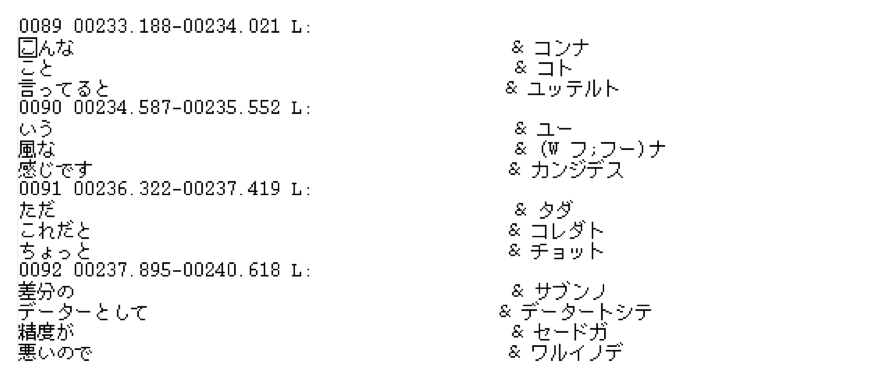
\includegraphics{./figure/kakiokosi.eps}
  \end{center}
  \caption{各話者クラスタに含まれる発話データ数 \label{fig:yoshimura_kikouzou}}
\end{figure}

本実験で使用した音響モデル、言語モデル、単語辞書の仕様は\ref{section:experiment_acoustic_model}節、\ref{section:experiment_language_model}節で述べる。

\subsection{音響モデルの仕様}
\label{section:experiment_acoustic_model}
本実験で用いたDNN-HMM音響モデルの仕様を表\ref{table:acoustic_model_detail}に示す。この仕様に関しては小島らの研究\cite{kojima}で使用されたもので、状態数は3000、音響特徴の次元数は39次元(表\ref{acoustic_model_feature})、隠れ層の数は6層、各層における繰り返し学習数は5回、隠れ層のノード数は1024とした。以下に、DNNを用いた際の学習の手順を示す。

\begin{table}[H]
  \begin{center}
    \caption{音響モデルの仕様 \label{table:acoustic_model_detail}}
    \begin{tabular}{|c|c|c|} \hline
     状態数  & 使用した音素 & 混合数 \\ \hline
     3,000  & 27 & 16 \\ \hline
    \end{tabular}
  \end{center}
\end{table}

\begin{table}[H]
  \begin{center}
    \caption{使用する音響特徴パラメータ \label{acoustic_model_feature}}
    \begin{tabular}{|c||c|} \hline
      特徴量 & 次元数\\ \hline
      MFCC & 12  \\ \hline
      POW & 1  \\ \hline
      $\Delta$MFCC & 12 \\ \hline
      $\Delta$POW & 1 \\ \hline
      $\Delta\Delta$MFCC & 12 \\ \hline
      $\Delta\Delta$POW & 1 \\ \hline
      計 & 39 \\ \hline
    \end{tabular}
  \end{center}
\end{table}

\vspace{0.2in}\noindent{\textbf{\underline{構築手順}}}\par
DNNを用いた音響モデルの構築や、この音響モデルを用いた音声認識に必要な学習テキストや言語モデルを作成する為にKaldiツールキットを用いた\cite{kaldi}。このツールキットの大きな流れを図\ref{fig:flow_train_dnn}に示す。まず学習や評価に必要なデータを用意し、言語モデルと単語辞書のWeighted Finite State Transducer (WFST)を作成する。WFSTとは重み付き有限トランスデューサといい、状態遷移機械モデル有限オートマトンの一種である。次に音声データから特徴量を抽出したデータを準備し、このデータと書き起こしを用いてGMM-HMMによる音響モデルのWFSTを作成する。これらのWFSTを、合成等を行ない1つのWFSTとする。このWFSTを用いて音声認識を行ない、学習データのアライメント(フレームごとの音素情報)をとる。このアライメントを用いてDNNを用いた音響モデルの学習(プレトレーニングと微調整)を行ない、最終的な音声認識を行なう。

\begin{figure}[H]
  \begin{center}
    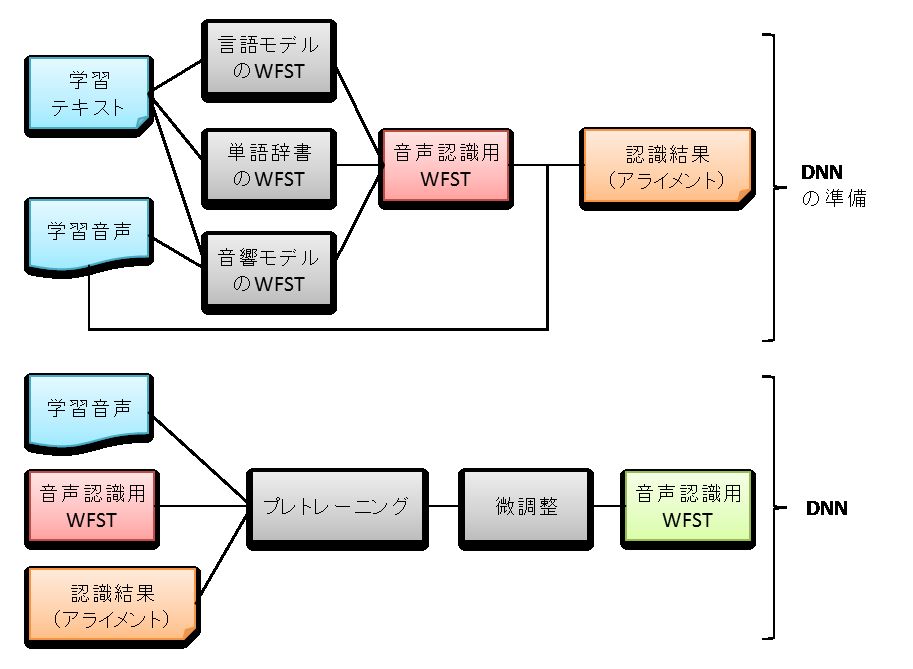
\includegraphics{./figure/flow_train_dnn.eps}
  \end{center}
  \caption{DNNを用いる際の学習の流れ \label{fig:flow_train_dnn}}
\end{figure}

\vspace{0.2in}\noindent{\textbf{\underline{木構造話者クラスタ}}}\par
先行研究\cite{yoshimura_clustering}では、話者の音響特徴、話者特徴ごとに作成した木構造話者クラスタ、音響モデルを作成することで音声認識精度の向上を確認したため、本研究でも使用する。このクラスタは、母音の定常状態であるHMMの中央の状態の平均と分散を用いたBhattacharyya距離によるk-means法によって作成した。クラスタの個数は、最上位のクラスタを2分割し、作成された2つのクラスタをさらに2分割した計7つのクラスタを使用する。


\subsection{言語モデル・単語辞書の仕様}
\label{section:experiment_language_model}
言語モデルはトライグラムモデルを構築した。以下、使用した学習テキストを説明する。

\vspace{0.2in}\noindent{\textbf{\underline{CSJ}}}\par
CSJには書き起こしテキストも提供されており、その一部の例を図\ref{fig:kakiokosi}に示す。書き起こしテキストは主に情報部と発話部に区別される。情報部では発話IDや時間情報等を、発話部では発話内容を「&」の左側に基本形、右側に発音形という形式で記している。発話形はカタカナを用いて実際に発音された音声を忠実に表記したものである。発音の怠けや言い間違い等を書き取れる範囲で忠実に記録している。本研究では、音響モデル構築の際には主に発話部の発音形を用い、このカタカナ表記を音素列に変換し、ラベルファイルとして定義する。
\begin{figure}[H]
  \begin{center}
    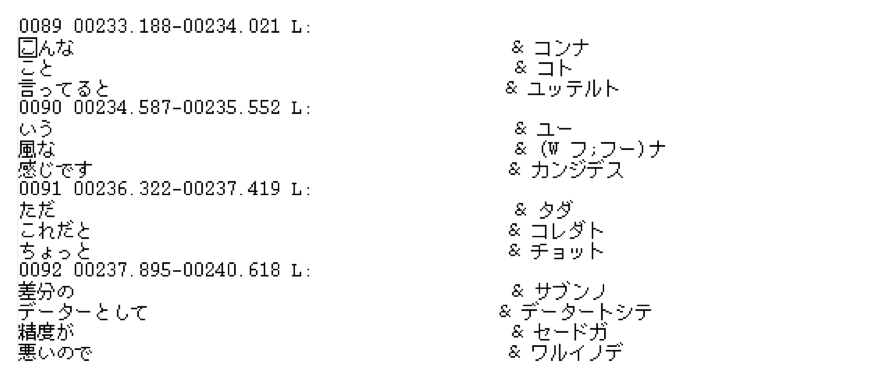
\includegraphics{./figure/kakiokosi.eps}
  \end{center}
  \caption{書き起こしテキストの例 \label{fig:kakiokosi}}
\end{figure}

本研究ではこのCSJをベースに学習テキストを構成する。使用するデータは977講演分のテキストで、約14MBである。

\vspace{0.2in}\noindent{\textbf{\underline{拡張したコーパスによる学習テキスト}}}\par
この学習テキストは江頭らによる、学術講演の書き起こしと新聞記事に拡張されるテキストとして参加者名の入ったテキスト、Webから収集してきたテキスト、そして対話コーパスから作成される対話テキストを追加した未知語の減少に着目した学習テキストである。この学習テキストは会議中に参加者の名前を呼ぶことが多い、会議は対話形式であるなどの会議の特徴を考慮した学習テキストである。テキストサイズは約100MBである。以降本論文では、このテキストを拡張したコーパスによる学習テキストと呼ぶ。

\vspace{0.2in}\noindent{\textbf{\underline{拡張したコーパスによる学習テキスト}}}\par
この学習テキストは荒井らによる、会議における発話行為に着目して作成された学習テキストである。学術講演の書き起こしと新聞記事に対話表現に近い特徴を持っていると考えられるQ&Aサイトから収集したテキストと対話コーパスを追加した学習テキストである。テキストサイズは約44MBである。以降本論文ではこのテキストを対話特化テキストと呼ぶ。


\subsection{評価方法}
本研究では評価尺度としては式\ref{calc:word_acc}で与えられる単語正解精度$Acc$(Word Accuracy)を用いる。ここで$W$は単語数、$S$(Substitution)は置換誤り、$D$(Deletion)は脱落誤り、$I$(Insertions)は挿入誤りの単語数を表わす。置換誤りとは、正解の単語が別の単語に誤認識された場合の誤りである。脱落誤りとは、単語があるべき部分に認識結果が何も出力されなかった場合の誤りである。挿入誤りは、本来単語がない部分に誤認識結果として単語が出力された場合の誤りである。

\begin{equation}
\label{calc:word_acc}
Acc=\frac{(W-S-D-I)}{W}
\end{equation}

          
評価は、正解ファイルと認識結果のファイルをDPマッチングを行なうことにより算出する。この正解ファイルは形態素解析した結果の形態素列によって作成したものである。
また、本研究ではアンカーの発話区間を対象とした音声認識を行うため、\ref{chapter:get_anchor}章で検出した発話区間より、アンカー以外の発話区間で認識された単語は全て挿入誤り、アンカーの発話として検出出来なかった発話区間の単語は全て削除誤りとして計算する。
\subsection{実験結果}
\subsection{考察}
  % 音声認識実験

   % 基礎理論
\chapter{予備調査}
\chapter{ニュース番組音声における発話の間隔の調査}
本章では、ニュース番組音声の発話間隔の調査を行う。これは、同一話者が連続で発話する場合は次の発話までの間隔が非常に短いと考え、話者が切り替わる際は、映像の切り替わりなどがあるため発話の間隔が長いと考えた。\par
そのため、

\section{使用する音声データ}
パラメータの学習用にニュース番組の音声データ13個を用いる。各音声データには、事前に人手で4種類(音楽、音声、雑音、無音)の音源ラベルが付与されている。「音声」の音源ラベルが付与された区間においては、更に発話者の情報が付与されている。また「音声」の音源ラベルをもとに対象の音声データから発話区間を抽出し、それを一発話とした。\par
表\ref{table:train_detail}に検証に用いるデータの詳細を示す。\vspace{0.2in}

\begin{table}[htb]
  \begin{center}
  \label{table:train_detail}
    \caption{パラメータの学習用音声データの詳細}
    \begin{tabular}{|c||c|c|c|} \hline
      データID & 収録時間 & 話者数 & 全発話数 \\ \hline
      ニュースF & 30分3秒 & 20 & 337 \\ \hline
      ニュースG & 30分3秒 & 31 & 312\\ \hline
      ニュースH & 30分3秒 & 21 & 324 \\ \hline
      ニュースI & 30分4秒 & 20 & 324\\ \hline
      ニュースJ & 20分3秒 & 13 & 159\\ \hline
      ニュースK & 30分3秒 & 22 & 343\\ \hline
      ニュースL & 30分4秒 & 22 & 313\\ \hline
      ニュースM & 30分4秒 & 20 & 315\\ \hline
      ニュースN & 30分4秒 & 17 & 321\\ \hline
      ニュースO & 30分4秒 & 16 & 337\\ \hline
      ニュースP & 30分4秒 & 20 & 363\\ \hline
      ニュースQ & 30分4秒 & 26 & 345\\ \hline
      ニュースR & 30分4秒 & 26 & 314\\ \hline
    \end{tabular}
  \end{center}
\end{table}
\section{実験結果}
\section{コサイン類似度を用いたi-vectorの性質の調査}
\label{section:pre_cos}
\subsection{使用する音声データ}
\label{section:detail_ATR}
UBMモデルの学習データおよびコサイン類似度を用いたi-vectorの性質の調査に読み上げ音声\cite{ATR}を使用した。読み上げ音声には、男女各110人$×$50発話分が収録されている。

\subsection{調査方法}
各話者の音声データから1つの発話を取り出し、それ以外の音声データとのi-vectorのコサイン類似度を算出する。また、同一話者の発話間の場合と異なる話者の発話間の2つの場合で発話の長さごとのコサイン類似度が取る値の検証を行う。\par

\subsection{コサイン類似度の算出条件}
i-vectorの抽出には、ALIZEとLIR RAL\cite{alize}を用いる。読み上げ音声に収録されている各発話データからi-vectorを抽出する。発話データから抽出する音響特徴パラメータを表\ref{iv_feature}に示す。また混合数は32とした。

\begin{table}[H]
  \begin{center}
    \caption{使用する音響特徴パラメータ}
    \label{iv_feature}
    \begin{tabular}{|c||c|} \hline
      特徴量 & 次元数\\ \hline
      MFCC & 19  \\ 
      POW & 1  \\ 
      $\Delta$MFCC & 19 \\ 
      $\Delta$POW & 1 \\ 
      $\Delta\Delta$MFCC & 19 \\ 
      $\Delta\Delta$POW & 1 \\ \hline
      計 & 60 \\ \hline
    \end{tabular}
  \end{center}
\end{table}

本稿では、音響特徴量のひとつとしてメル周波数ケプストラム係数(MFCC)を用いる。メル周波数ケプストラム係数(Mel - Frequency Cepstrum Coefficient : MFCC)とは、メル周波数という人間の音の高低に対する感覚尺度を考慮した特徴量であり、音声スペクトルから係数スペクトルを抽出したものである。これは一般的に、音声の特徴を抽出するパラメータとして用いられる。[5]

\subsection{調査結果}
\noindent{\textbf{\underline{同一話者間のi-vectorの特徴}}}\par
同一話者間のi-vectorのコサイン類似度を図\ref{fig:same_cos_hist}、その標準偏差を図\ref{fig:same_cos_vari}に示す。\par

\begin{figure}[H]
  \begin{center}
    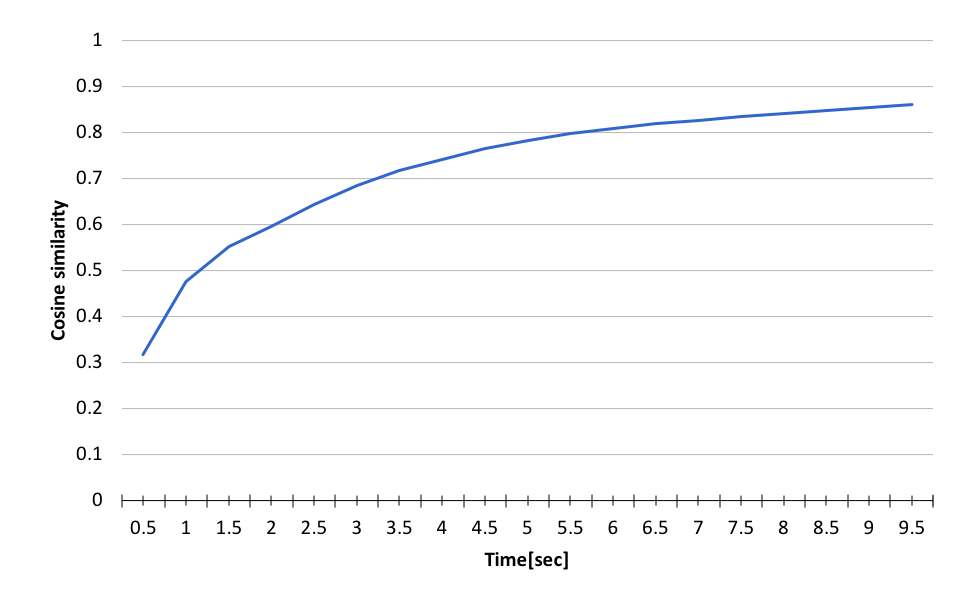
\includegraphics[scale=0.8]{./figure/same_cos_hist.eps}
  \end{center}
  \caption{同一話者間のi-vectorのコサイン類似度 \label{fig:same_cos_hist}}
\end{figure}

\begin{figure}[H]
  \begin{center}
    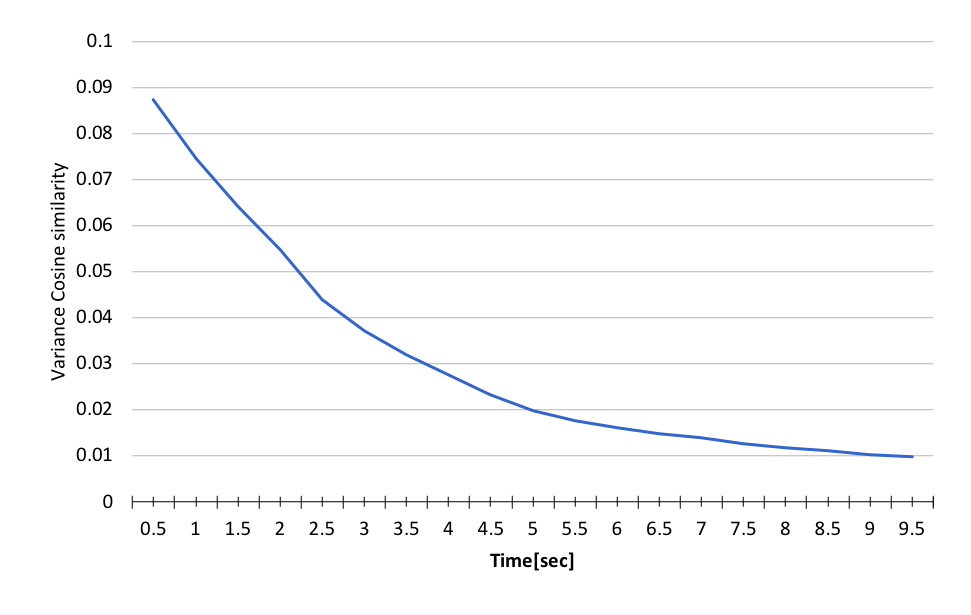
\includegraphics[scale=0.8]{./figure/same_cos_vari.eps}
  \end{center}
  \caption{同一話者間のi-vectorのコサイン類似度の標準偏差 \label{fig:same_cos_vari}}
\end{figure}

図\ref{fig:same_cos_hist}より、発話が長いほどコサイン類似度の値が高くなる傾向にある。また、図\ref{fig:same_cos_vari}より、発話が短い場合はコサイン類似度のばらつきが大きく、長くなるにつれて収束する傾向にある。\par


\vspace{0.2in}\noindent{\textbf{\underline{異なる話者間のi-vectorの特徴}}}\par
異なる話者間のi-vectorのコサイン類似度を図\ref{fig:other_cos_hist}、その標準偏差を図\ref{fig:other_cos_vari}に示す。\par

\begin{figure}[H]
  \begin{center}
    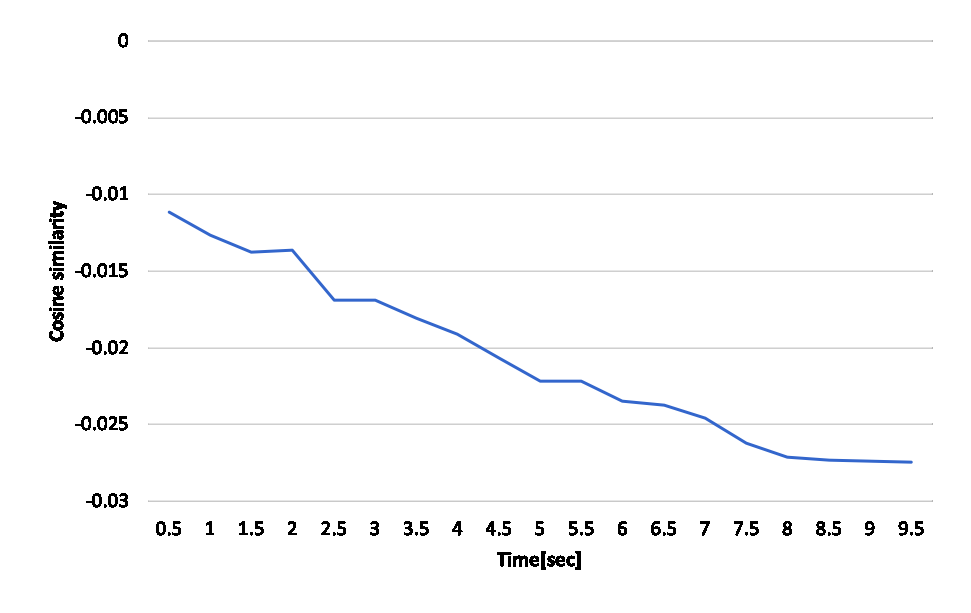
\includegraphics[scale=0.8]{./figure/other_cos_hist.eps}
  \end{center}
  \caption{異なる話者間のi-vectorのコサイン類似度 \label{fig:other_cos_hist}}
\end{figure}

\begin{figure}[H]
  \begin{center}
    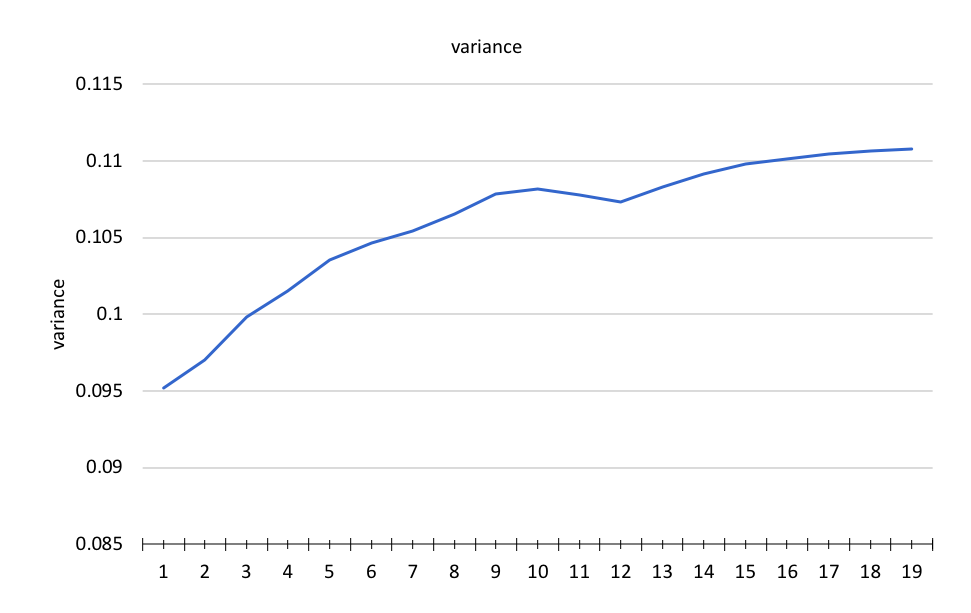
\includegraphics[scale=0.8]{./figure/other_cos_vari.eps}
  \end{center}
  \caption{異なる話者間のi-vectorのコサイン類似度の標準偏差 \label{fig:other_cos_vari}}
\end{figure}

図\ref{fig:other_cos_hist}より、発話が長くなるほどコサイン類似度が低くなる傾向にある。また、図\ref{fig:other_cos_vari}より、発話が長くなるごとにコサイン類似度のばらつきが大きくなる傾向にある。\par

\subsection{考察}
発話が短い時、同一話者間のコサイン類似度のばらつきが大きい理由として、短い発話からは話者の特徴が十分に抽出できていないためであると考えられる。また発話が短い時、異なる話者間のコサイン類似度のばらつきが小さいことから、話者の特徴を抽出できていない場合、話者が異なっていてもi-vectorのコサイン類似度が似た値をとることがわかる。つまり、i-vectorを用いた話者識別、話者照合を行う場合、できるだけ長い発話を用いる必要がある。
 %予備調査
%\chapter{i-vectorを用いたアンカーの発話区間検出手法および音声認識とその課題}

\section{i-vectorを用いたアンカーの発話区間検出手法}
\label{section:clustering}
先行研究\cite{nozaki_gakuseikai}では、i-vectorを用いてアンカーの発話区間の検出を行った。ニュース番組では、アンカー以外にインタビューイ(インタビューの受け手)や中継の有無によって話者数が大きく異なる。そのためクラスタ数を決定した場合、クラスタ数と話者数に不一致が起こり同一アンカーの発話群検出精度が低下する場合がある。そこで,同一話者の発話データのi-vectorはベクトル空間上で局所的に分布することに着目した。アンカーの発話数は非アンカーと比較して多いことから多くのアンカーの発話が局所的に集まると考えたため、同一アンカーの発話データをより精度よく検出できると考えた。\par
そこで、2つの発話データのi-vectorのコサイン類似度が閾値$Th_{cos}$以上の場合、その2つの発話データの話者は同一話者であると仮定した。まず、全ての発話データ間のi-vectorのコサイン類似度を求める。次に、このコサイン類似度が閾値$Th_{cos}$以上となる発話データ数が最も多い発話データを同一アンカーの発話データ群$O$のセントロイドとし、閾値$Th_{cos}$以上(話者性が類似している)の全データをそのデータ群$O$の初期要素とする。\par
一方、i-vectorを抽出する発話データの発声の抑揚が大きい場合、同一話者の発話間のi-vectorであってもコサイン類似度が閾値$Th_{cos}$以下になる場合がある。そこで、発話データ$u_i(\in O)$と発話データ群$O$の距離が一定距離以内であるとき、発話データ$u_i$は発話データ群$O$の要素として追加する。\par
以上の手法により、アンカーの発話区間検出精度の向上が確認された。

\section{i-vectorを用いた音声認識手法}
\label{section:yoshimura_pre_clustering}
先行研究\cite{yoshimura_clustering}では、学習データに含まれる話者の音響特徴、話者特徴ごとに作成した木構造話者クラスタ、音響モデルを作成した。このクラスタは、母音の定常状態であるHMMの中央の状態の平均と分散を用いたBhattacharyya距離によるk-means法によって作成した。クラスタの個数は、最上位のクラスタを2分割し、作成された2つのクラスタをさらに2分割した計7つのクラスタを使用する。\par
学習データに用いた話者のi-vectorと評価データのi-vectorのコサイン類似度を求める。求めたコサイン類似度の高い上位$n$人の学習データを全て含んでいるクラスタをその評価データを認識するクラスタとする。この手法では木構造話者クラスタの性質上、$n$人の学習データをすべて含んでいるクラスタが複数存在する可能性がある。その場合、より下層のクラスタの方が選択された話者の割合が高いため、より下層のクラスタを認識するクラスタとする。\par
以上の木構造話者クラスタにより作成された音響モデルで音声認識を行った結果、認識精度の向上が確認された。

\section{課題}
両手法ともに、i-vectorを用いることの有意性を示している。しかし、\ref{section:pre_cos}節でも述べた通り発話が非常に短い場合はi-vectorの抽出精度が低下する。そのため、アンカーの発話区間検出ではクラスタリングによる話者の識別が非常に困難となり、アンカーの発話区間の誤検出に繋がると考えられる。また音声認識では、認識対象の評価データと音響モデルを作成した話者クラスタに含まれる学習データとのコサイン類似度を計算して音響モデルを選択しているため、適切な音響モデルを選択できない可能性がある。
%\chapter{i-vectorの抽出精度向上のための発話区間結合手法}
\label{chapter:prob_method}
i-vectorを用いたアンカーの発話区間検出精度、音声認識精度は共にi-vectorの抽出精度によって大きく左右される。そこで、i-vector抽出精度向上のためにニュース番組特有の特徴である「対話表現が少ない」「同じ話者が連続で発話する」「様々な場所で発話する」の3点に着目した。これは、同じ話者の発話区間であると考えられる前後の発話区間を結合し、擬似的に長い発話を作成することでi-vectorの抽出精度の向上が見込めると考えたためである。そのため本稿では、2通りの方法で前後の同一話者と考えられる発話区間を結合する。1つ目は発話間の時間情報を考慮した発話区間の結合手法である。2つめは、話者の発話環境を考慮した発話区間の結合手法である。図\ref{fig:indexing2}は、本稿の提案手法を組み込んだインデクシング手法の流れである。

\begin{figure}[H]
  \begin{center}
    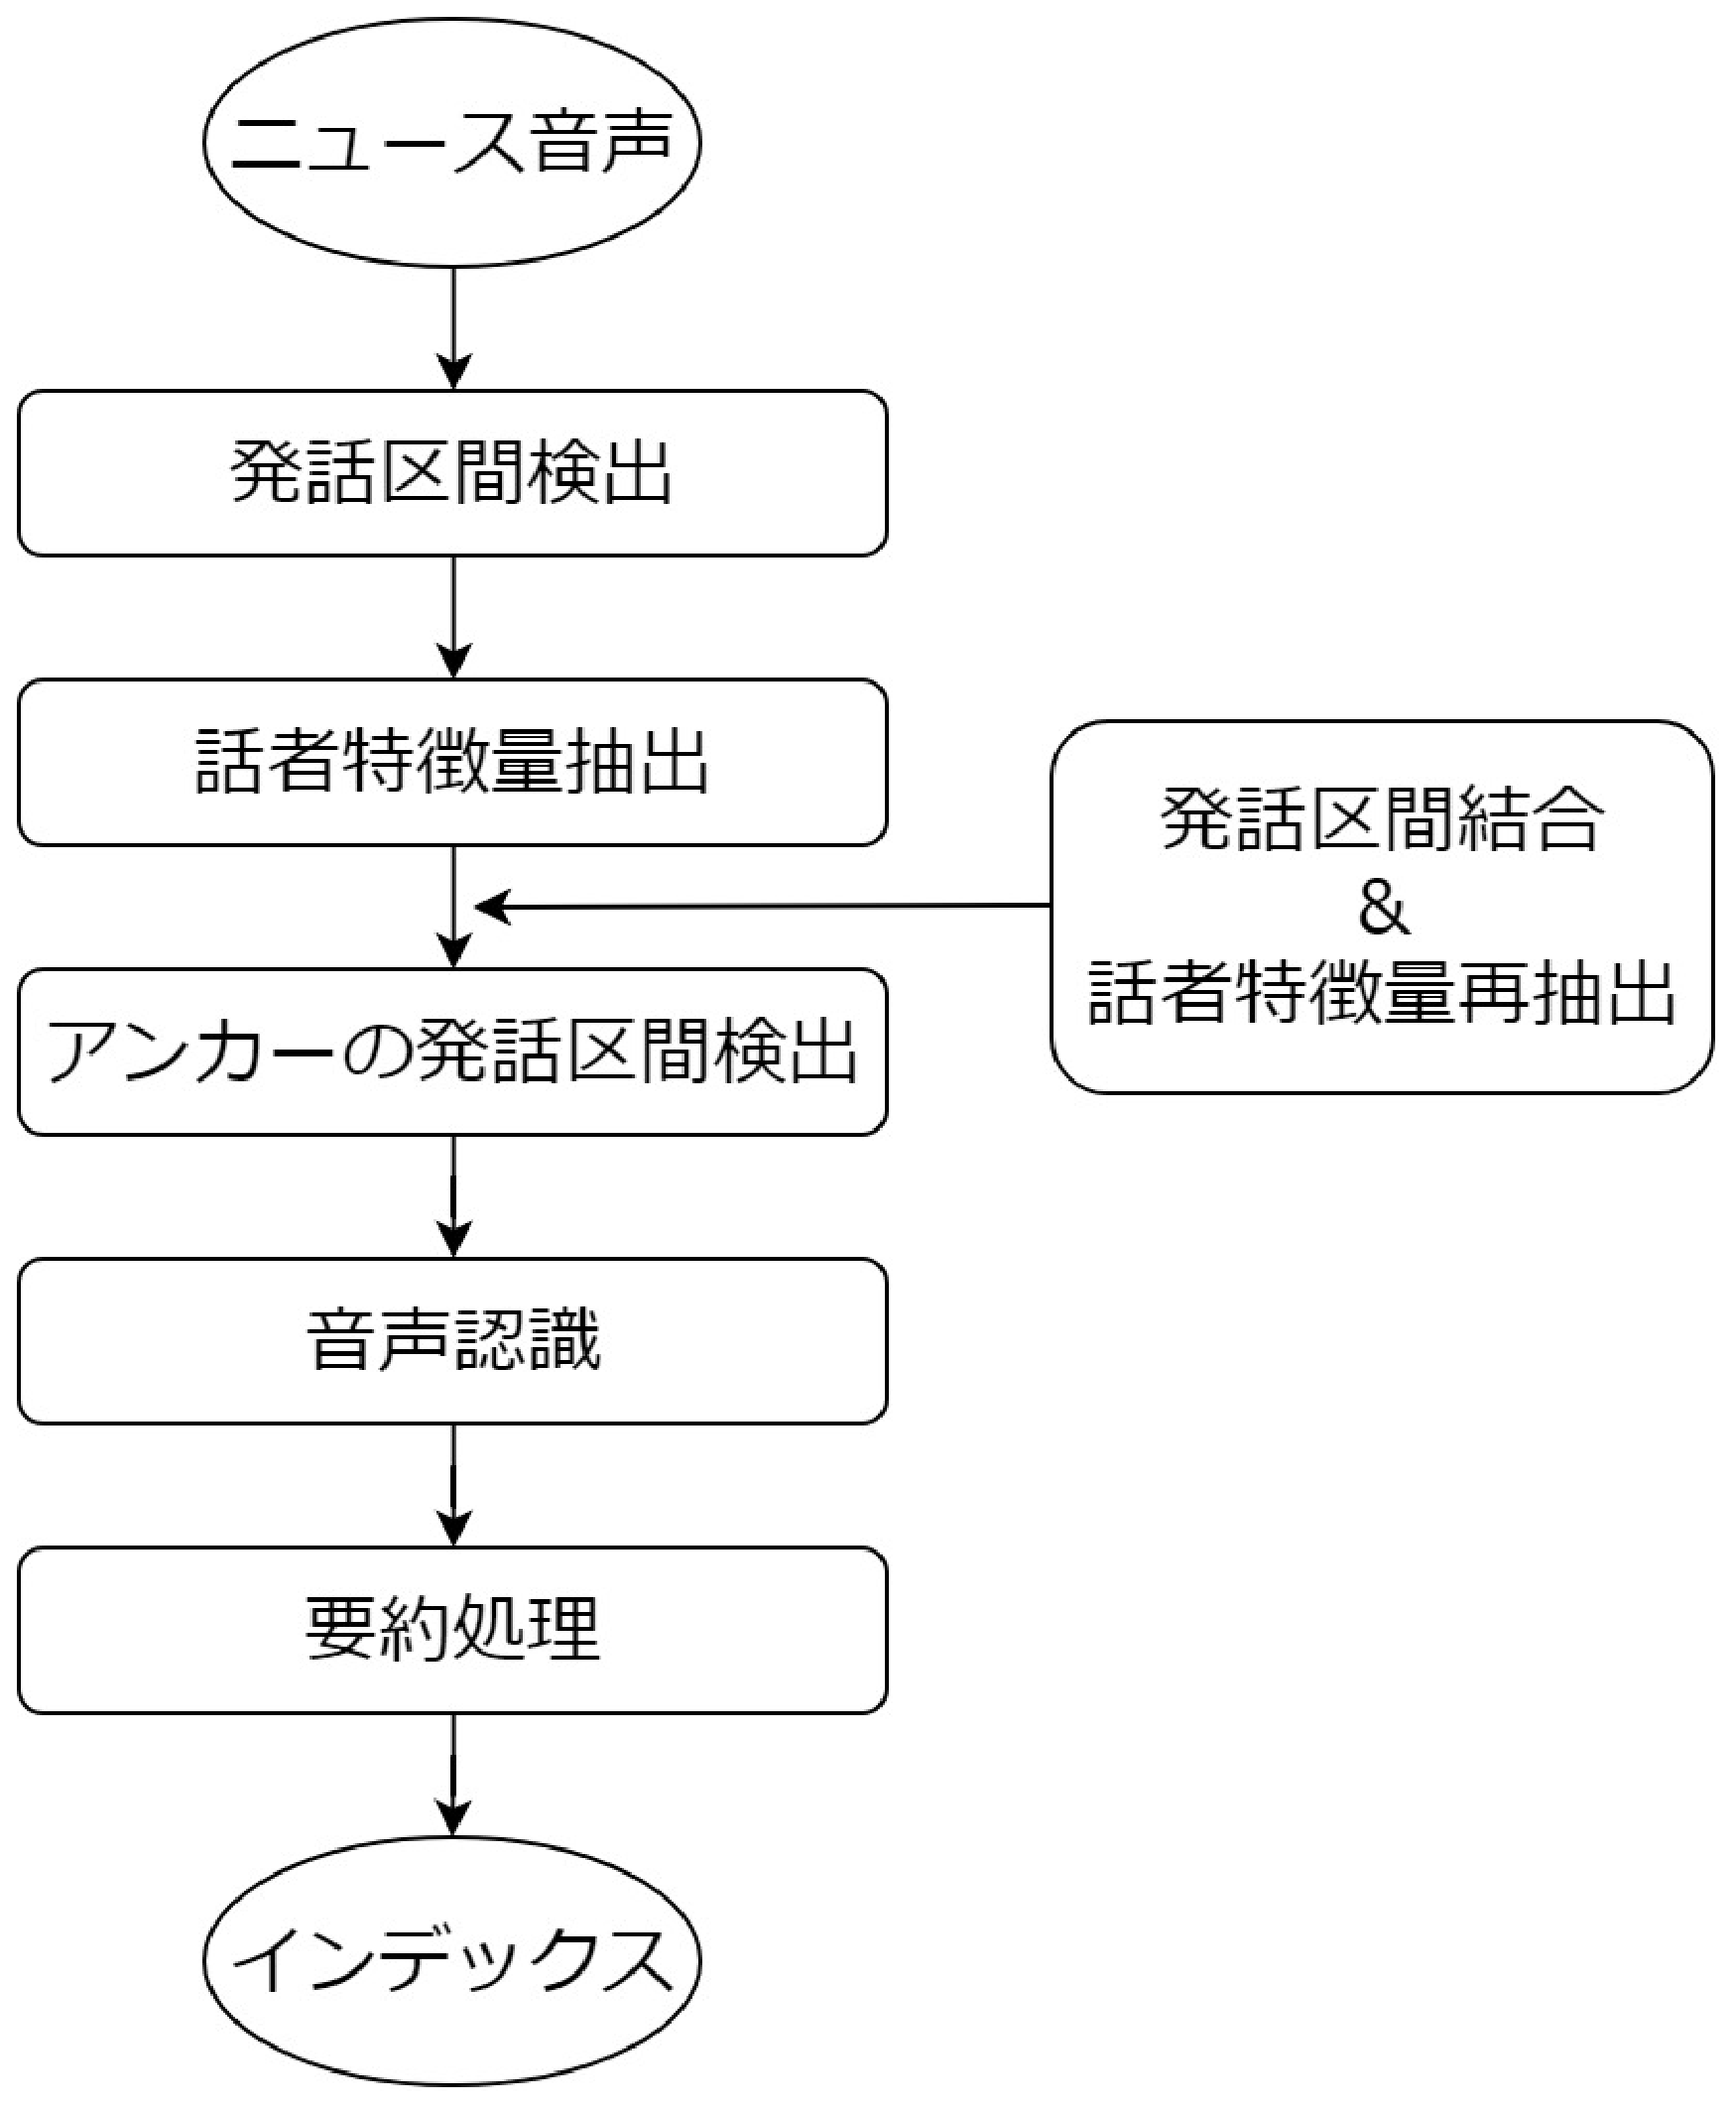
\includegraphics[scale=0.3]{./figure/indexing2.eps}
  \end{center}
  \caption{提案手法を組み込んだインデクシング手法 \label{fig:indexing2}}
\end{figure}

\section{発話間の時間情報を考慮した発話区間の結合手法}
本手法では、発話区間と発話区間の間(非発話区間)が短い場合、発話区間を結合する。これは図\ref{fig:same_sp}で示されるように、同一話者が連続で発話する場合は間をおかずに次の発話を行うことが非常に多いためである。つまり、非発話区間が非常に短いとき、高い確率で同一話者の発話が行われる。そこで、非発話区間が非常に短い場合、同一話者の発話と判別し発話区間を結合する。しかし、\ref{fig:different_sp}でもあるように、話者が切り替わった場合でも非発話区間が短い場合がある。このため、非発話区間の長さのみで結合した場合、異なる話者同士で発話区間を結合してしまい、i-vectorの抽出に悪影響がある。そこで、コサイン類似度の閾値$Th_{cos}$を設ける。非発話区間が非常に短く、その非発話区間を挟んでいる発話区間から抽出したi-vectorのコサイン類似度が一定値以上の時、同一話者同士の発話区間であるとして発話区間を結合する。

\section{発話環境を考慮した発話区間の結合手法}
本手法では発話環境を音源識別によって検出し、発話環境の変化を検出した場合、同一話者の可能性が高いとして前後の発話区間を結合する。ニュース番組にはスタジオにいるアンカーのほか、台風の状況を中継する中継アナウンサー、騒音の中でインタビューを受けるインタビューイなどが存在する。例えば、アンカーから中継アナウンサー、インタビューイからアンカーなど話者が切り替わった場合、発話環境が変化する。本稿で使用する音源識別システムはニュース番組音声を「音声」「背景雑音」「音楽」「無音」のいずれかに分類する。そのため、「音声」以外の区間、つまり非発話区間の音源識別結果である「背景雑音」「音楽」「無音」の検出結果が変化した時発話環境の変化したと識別することができる。以上の理由により、発話環境が変化するまでの範囲で発話している話者を同一話者として発話区間を結合する。\par
 % 提案手法
%\chapter{実験}
\section{使用する音声データ}
評価用にニュース番組の音声データ5個を用いる。本来のニュース番組の音声には「音声」の音源ラベルが付与されていない。そこで、音源識別を用いて発話区間を検出、切り出しを行なった。また、切り出された発話区間それぞれを一発話し、各発話区間に人手で発話者の情報が付与した。\par
表\ref{table:test_detail}に検証に用いるデータの詳細、表\ref{table:test_detail_RPF}に音源識別による発話区間検出精度を示す。

\begin{table}[H]
  \begin{center}
    \caption{評価用音声データの詳細 \label{table:test_detail}}
    \begin{tabular}{|c||c|c|c|} \hline
      データID & 収録時間 & 話者数 & 全発話数 \\ \hline
      ニュース1 & 30分3秒 & 20 & 337 \\ \hline
      ニュース2 & 30分3秒 & 31 & 312\\ \hline
      ニュース3 & 30分3秒 & 21 & 324 \\ \hline
      ニュース4 & 30分4秒 & 20 & 324\\ \hline
      ニュース5 & 20分3秒 & 13 & 159\\ \hline
    \end{tabular}
  \end{center}
\end{table}

\begin{table}[H]
  \begin{center}
    \caption{評価用音声データの発話区間検出精度$[\%]$ \label{table:test_detail_RPF}}
    \begin{tabular}{|c||c|c|c|} \hline
      データID & Recall & Precision & F-meature \\ \hline
      ニュース1 & 89.49 & 91.60 & 90.53 \\ \hline
      ニュース2 & 84.09 & 95.54 & 89.45\\ \hline
      ニュース3 & 88.30 & 85.99 & 87.13 \\ \hline
      ニュース4 & 90.06 & 83.33 & 86.56\\ \hline
      ニュース5 & 90.95 & 90.30 & 90.63\\ \hline
    \end{tabular}
  \end{center}
\end{table}

\chapter{発話区間の結合実験}
本章では、ニュース番組音声の発話区間を対象として、前後の発話区間が同一話者である可能性が高いとき発話区間を結合する。
\section{実験方法}
ニュース番組内の発話区間から予め
\section{使用する音声データ}
\noindent{\textbf{\underline{評価用音声データ}}}\par
評価用にニュース番組の音声データ5個を用いる。本来のニュース番組の音声には「音声」の音源ラベルが付与されていない。そこで、音源識別を用いて発話区間を検出、切り出しを行なった。また、切り出された発話区間それぞれを一発話し、各発話区間に人手で発話者の情報が付与した。\par
表\ref{table:test_detail}に検証に用いるデータの詳細、表\ref{table:train_detail_RPF}に音源識別による発話区間検出精度を示す。

\begin{table}[htb]
  \begin{center}
  \label{table:test_detail}
    \caption{評価用音声データの詳細}
    \begin{tabular}{|c||c|c|c|} \hline
      データID & 収録時間 & 話者数 & 全発話数 \\ \hline
      ニュースA & 30分3秒 & 20 & 337 \\ \hline
      ニュースB & 30分3秒 & 31 & 312\\ \hline
      ニュースC & 30分3秒 & 21 & 324 \\ \hline
      ニュースD & 30分4秒 & 20 & 324\\ \hline
      ニュースE & 20分3秒 & 13 & 159\\ \hline
    \end{tabular}
  \end{center}
\end{table}

\begin{table}[htb]
  \begin{center}
  \label{table:test_detail}
    \caption{評価用音声データの発話区間検出精度$[\%]$}
    \begin{tabular}{|c||c|c|c|} \hline
      データID & Recall & Precision & F-meature \\ \hline
      ニュースA & 89.49 & 91.60 & 90.53 \\ \hline
      ニュースB & 84.09 & 95.54 & 89.45\\ \hline
      ニュースC & 88.30 & 85.99 & 87.13 \\ \hline
      ニュースD & 90.06 & 83.33 & 86.56\\ \hline
      ニュースE & 90.95 & 90.30 & 90.63\\ \hline
    \end{tabular}
  \end{center}
\end{table}

\noindent{\textbf{\underline{パラメータの学習用音声データ}}}\par
パラメータの学習用にニュース番組の音声データ13個を用いる。各音声データには、事前に人手で4種類(音楽、音声、雑音、無音)の音源ラベルが付与されている。「音声」の音源ラベルが付与された区間においては、更に発話者の情報が付与されている。また「音声」の音源ラベルをもとに対象の音声データから発話区間を抽出し、それを一発話とした。\par
表\ref{table:train_detail}に検証に用いるデータの詳細を示す。\vspace{0.2in}

\begin{table}[htb]
  \begin{center}
  \label{table:train_detail}
    \caption{パラメータの学習用音声データの詳細}
    \begin{tabular}{|c||c|c|c|} \hline
      データID & 収録時間 & 話者数 & 全発話数 \\ \hline
      ニュースF & 30分3秒 & 20 & 337 \\ \hline
      ニュースG & 30分3秒 & 31 & 312\\ \hline
      ニュースH & 30分3秒 & 21 & 324 \\ \hline
      ニュースI & 30分4秒 & 20 & 324\\ \hline
      ニュースJ & 20分3秒 & 13 & 159\\ \hline
      ニュースK & 30分3秒 & 22 & 343\\ \hline
      ニュースL & 30分4秒 & 22 & 313\\ \hline
      ニュースM & 30分4秒 & 20 & 315\\ \hline
      ニュースN & 30分4秒 & 17 & 321\\ \hline
      ニュースO & 30分4秒 & 16 & 337\\ \hline
      ニュースP & 30分4秒 & 20 & 363\\ \hline
      ニュースQ & 30分4秒 & 26 & 345\\ \hline
      ニュースR & 30分4秒 & 26 & 314\\ \hline
    \end{tabular}
  \end{center}
\end{table}


\section{実験結果}
    % 発話区間の結合実験
\section{アンカーの発話群検出実験}
本節では、i-vectorを用いてアンカーの発話区間検出を行う。
\label{chapter:get_anchor}
\subsection{実験方法}
本節では、\ref{chapter:connect_sp}節の手法1で得られたi-vectorを用いてアンカーの発話区間検出を行う。i-vectorを用いたアンカーの発話区間抽出方法を\ref{section:clustering}節に示す。

\subsection{評価方法}
評価は、検出されたアンカーの発話区間と正解ラベルを比較して行う。

\begin{table}[H]
\begin{center}
    \caption{アンカーの発話区間の正誤判定 \label{table:clustering}}
\begin{tabular}{|c|c|c|c|l}
\cline{1-4}
\multicolumn{2}{|c|}{\multirow{2}{*}{}} & \multicolumn{2}{c|}{「発話者」のラベルが付与された発話区間} &  \\ \cline{3-4}
\multicolumn{2}{|c|}{}                  & アンカーの発話区間        & アンカー以外の発話区間        &  \\ \cline{1-4}
\multirow{2}{*}{判定結果}        & 正        & $TP$                  & $FP$                   &  \\ \cline{2-4}
& 誤        & $FN$                  & $TN$                   &  \\ \cline{1-4}
\end{tabular}
\end{center}
\end{table}

表\ref{table:clustering}を用いて、$P$(適合率(Precision))と$R$(再現率(Recall))を式\ref{calc:precision2}と式\ref{calc:recall2}のようにそれぞれ定義する。また、$F$値($F-measure$)を式\ref{calc:fmeasure2}のように定義する。

\begin{equation}
\label{calc:precision2}
P = \frac{TP}{TP + FP}
\end{equation}

\begin{equation}
\label{calc:recall2}
R = \frac{TP}{TP + FN}
\end{equation}

\begin{equation}
\label{calc:fmeasure2}
F = \frac{1}{\frac{1}{P} + \frac{1}{R}}
\end{equation}

ここで$P$と$R$はそれぞれ適合率、再現率を表す。

また、検出したアンカーの発話区間の割合を式\ref{calc:anchor_acc}のように定義して評価する。

\begin{equation}
\label{calc:anchor_acc}
Acc_{time} = \frac{検出したアンカーの発話区間の時間数}{アンカーの発話区間の時間数}
\end{equation}

本実験では、評価方法として適合率、再現率、$F$値、$Acc_{time}$を用いる。

\subsection{実験結果}
アンカーの発話区間検出精度を以下に示す。

\begin{table}[H]
  \begin{center}
    \caption{アンカーの発話区間検出精度($Th_{time}=0.8)$ \label{table:result_get_anchor08}}
    \begin{tabular}{|c||c|c|c|c|} \hline
      $Th_{cos}$ & $Recall$ & $Precision$ & $F-measure$ & $Acc_{time}$\\ \hline
0.5 & 0.836 & 0.632 & 0.72 & 0.794 \\ \hline
0.6 & 0.812 & 0.768 & 0.789 & 0.774 \\ \hline
0.7 & 0.778 & 0.866 & 0.82 & 0.747 \\ \hline
0.8 & 0.656 & 0.92 & 0.766 & 0.655 \\ \hline

    \end{tabular}
  \end{center}
\end{table}

\begin{table}[H]
  \begin{center}
    \caption{アンカーの発話区間検出精度($Th_{time}=0.9$) \label{table:result_get_anchor09}}
    \begin{tabular}{|c||c|c|c|c|} \hline
      $Th_{cos}$ & $Recall$ & $Precision$ & $F-measure$ & $Acc_{time}$\\ \hline
0.5 & 0.839 & 0.636 & 0.723 & 0.794 \\ \hline
0.6 & 0.81 & 0.775 & 0.792 & 0.771 \\ \hline
0.7 & 0.782 & 0.865 & 0.821 & 0.747 \\ \hline
0.8 & 0.681 & 0.915 & 0.781 & 0.671 \\ \hline

    \end{tabular}
  \end{center}
\end{table}

\begin{table}[H]
  \begin{center}
    \caption{アンカーの発話区間検出精度($Th_{time}=1.0$) \label{table:result_get_anchor10}}
    \begin{tabular}{|c||c|c|c|c|} \hline
      $Th_{cos}$ & $Recall$ & $Precision$ & $F-measure$ & $Acc_{time}$\\ \hline
0.5 & 0.837 & 0.638 & 0.724 & 0.793 \\ \hline
0.6 & 0.811 & 0.764 & 0.787 & 0.768 \\ \hline
0.7 & 0.784 & 0.867 & 0.824 & 0.747 \\ \hline
0.8 & 0.683 & 0.912 & 0.781 & 0.668 \\ \hline

    \end{tabular}
  \end{center}
\end{table}

\begin{table}[H]
  \begin{center}
    \caption{アンカーの発話区間検出精度($Th_{time}=1.1$) \label{table:result_get_anchor11}}
    \begin{tabular}{|c||c|c|c|c|} \hline
      $Th_{cos}$ & $Recall$ & $Precision$ & $F-measure$ & $Acc_{time}$\\ \hline
0.5 & 0.84 & 0.609 & 0.706 & 0.793 \\ \hline
0.6 & 0.815 & 0.714 & 0.761 & 0.772 \\ \hline
0.7 & 0.773 & 0.871 & 0.819 & 0.74 \\ \hline
0.8 & 0.688 & 0.91 & 0.783 & 0.675 \\ \hline

    \end{tabular}
  \end{center}
\end{table}


\begin{table}[H]
  \begin{center}
    \caption{アンカーの発話区間検出精度($Th_{time}=1.2$) \label{table:result_get_anchor12}}
    \begin{tabular}{|c||c|c|c|c|} \hline
      $Th_{cos}$ & $Recall$ & $Precision$ & $F-measure$ & $Acc_{time}$\\ \hline
0.5 & 0.841 & 0.587 & 0.692 & 0.793 \\ \hline
0.6 & 0.811 & 0.734 & 0.771 & 0.768 \\ \hline
0.7 & 0.774 & 0.877 & 0.822 & 0.741 \\ \hline
0.8 & 0.687 & 0.907 & 0.782 & 0.673 \\ \hline

    \end{tabular}
  \end{center}
\end{table}

\begin{table}[H]
  \begin{center}
    \caption{アンカーの発話区間検出精度($Th_{time}=1.3$) \label{table:result_get_anchor13}}
    \begin{tabular}{|c||c|c|c|c|} \hline
      $Th_{cos}$ & $Recall$ & $Precision$ & $F-measure$ & $Acc_{time}$\\ \hline
0.5 & 0.841 & 0.589 & 0.693 & 0.793 \\ \hline
0.6 & 0.809 & 0.699 & 0.75 & 0.769 \\ \hline
0.7 & 0.776 & 0.868 & 0.819 & 0.741 \\ \hline
0.8 & 0.686 & 0.902 & 0.779 & 0.672 \\ \hline

    \end{tabular}
  \end{center}
\end{table}

\begin{table}[H]
  \begin{center}
    \caption{アンカーの発話区間検出精度($Th_{time}=1.4$) \label{table:result_get_anchor14}}
    \begin{tabular}{|c||c|c|c|c|} \hline
      $Th_{cos}$ & $Recall$ & $Precision$ & $F-measure$ & $Acc_{time}$\\ \hline


    \end{tabular}
  \end{center}
\end{table}

\begin{table}[H]
  \begin{center}
    \caption{アンカーの発話区間検出精度($Th_{time}=1.5$) \label{table:result_get_anchor15}}
    \begin{tabular}{|c||c|c|c|c|} \hline
      $Th_{cos}$ & $Recall$ & $Precision$ & $F-measure$ & $Acc_{time}$\\ \hline


    \end{tabular}
  \end{center}
\end{table}
\subsection{考察}
  % アンカーの発話群検出実験
\section{アンカーの発話区間の音声認識実験}

\subsection{実験方法}
本実験では、\ref{section:yoshimura_pre_clustering}節で述べた話者クラスタを作成、音響モデルを作成して音声認識実験を行う。各話者クラスタに含まれる男女の発話データ数を図\ref{fig:yoshimura_kikouzou}に示す。

\begin{figure}[H]
  \begin{center}
    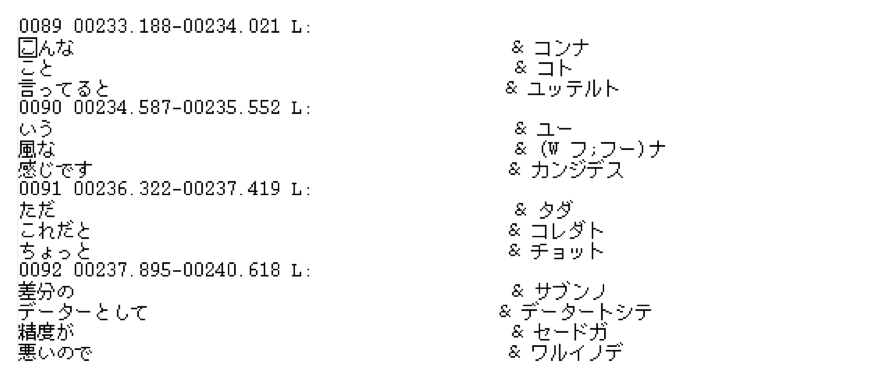
\includegraphics{./figure/kakiokosi.eps}
  \end{center}
  \caption{各話者クラスタに含まれる発話データ数 \label{fig:yoshimura_kikouzou}}
\end{figure}

本実験で使用した音響モデル、言語モデル、単語辞書の仕様は\ref{section:experiment_acoustic_model}節、\ref{section:experiment_language_model}節で述べる。

\subsection{音響モデルの仕様}
\label{section:experiment_acoustic_model}
本実験で用いたDNN-HMM音響モデルの仕様を表\ref{table:acoustic_model_detail}に示す。この仕様に関しては小島らの研究\cite{kojima}で使用されたもので、状態数は3000、音響特徴の次元数は39次元(表\ref{acoustic_model_feature})、隠れ層の数は6層、各層における繰り返し学習数は5回、隠れ層のノード数は1024とした。以下に、DNNを用いた際の学習の手順を示す。

\begin{table}[H]
  \begin{center}
    \caption{音響モデルの仕様 \label{table:acoustic_model_detail}}
    \begin{tabular}{|c|c|c|} \hline
     状態数  & 使用した音素 & 混合数 \\ \hline
     3,000  & 27 & 16 \\ \hline
    \end{tabular}
  \end{center}
\end{table}

\begin{table}[H]
  \begin{center}
    \caption{使用する音響特徴パラメータ \label{acoustic_model_feature}}
    \begin{tabular}{|c||c|} \hline
      特徴量 & 次元数\\ \hline
      MFCC & 12  \\ \hline
      POW & 1  \\ \hline
      $\Delta$MFCC & 12 \\ \hline
      $\Delta$POW & 1 \\ \hline
      $\Delta\Delta$MFCC & 12 \\ \hline
      $\Delta\Delta$POW & 1 \\ \hline
      計 & 39 \\ \hline
    \end{tabular}
  \end{center}
\end{table}

\vspace{0.2in}\noindent{\textbf{\underline{構築手順}}}\par
DNNを用いた音響モデルの構築や、この音響モデルを用いた音声認識に必要な学習テキストや言語モデルを作成する為にKaldiツールキットを用いた\cite{kaldi}。このツールキットの大きな流れを図\ref{fig:flow_train_dnn}に示す。まず学習や評価に必要なデータを用意し、言語モデルと単語辞書のWeighted Finite State Transducer (WFST)を作成する。WFSTとは重み付き有限トランスデューサといい、状態遷移機械モデル有限オートマトンの一種である。次に音声データから特徴量を抽出したデータを準備し、このデータと書き起こしを用いてGMM-HMMによる音響モデルのWFSTを作成する。これらのWFSTを、合成等を行ない1つのWFSTとする。このWFSTを用いて音声認識を行ない、学習データのアライメント(フレームごとの音素情報)をとる。このアライメントを用いてDNNを用いた音響モデルの学習(プレトレーニングと微調整)を行ない、最終的な音声認識を行なう。

\begin{figure}[H]
  \begin{center}
    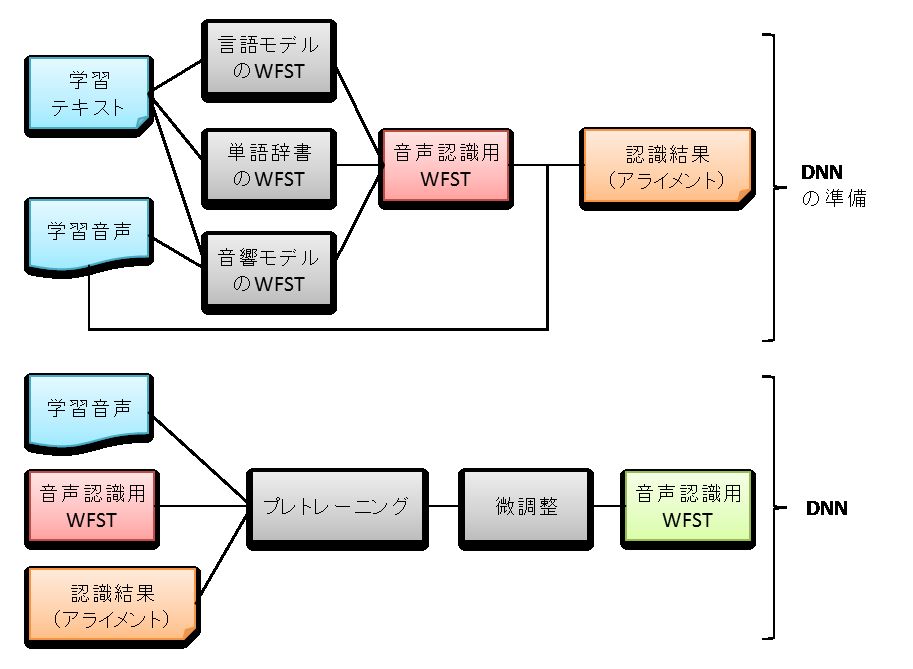
\includegraphics{./figure/flow_train_dnn.eps}
  \end{center}
  \caption{DNNを用いる際の学習の流れ \label{fig:flow_train_dnn}}
\end{figure}

\vspace{0.2in}\noindent{\textbf{\underline{木構造話者クラスタ}}}\par
先行研究\cite{yoshimura_clustering}では、話者の音響特徴、話者特徴ごとに作成した木構造話者クラスタ、音響モデルを作成することで音声認識精度の向上を確認したため、本研究でも使用する。このクラスタは、母音の定常状態であるHMMの中央の状態の平均と分散を用いたBhattacharyya距離によるk-means法によって作成した。クラスタの個数は、最上位のクラスタを2分割し、作成された2つのクラスタをさらに2分割した計7つのクラスタを使用する。


\subsection{言語モデル・単語辞書の仕様}
\label{section:experiment_language_model}
言語モデルはトライグラムモデルを構築した。以下、使用した学習テキストを説明する。

\vspace{0.2in}\noindent{\textbf{\underline{CSJ}}}\par
CSJには書き起こしテキストも提供されており、その一部の例を図\ref{fig:kakiokosi}に示す。書き起こしテキストは主に情報部と発話部に区別される。情報部では発話IDや時間情報等を、発話部では発話内容を「&」の左側に基本形、右側に発音形という形式で記している。発話形はカタカナを用いて実際に発音された音声を忠実に表記したものである。発音の怠けや言い間違い等を書き取れる範囲で忠実に記録している。本研究では、音響モデル構築の際には主に発話部の発音形を用い、このカタカナ表記を音素列に変換し、ラベルファイルとして定義する。
\begin{figure}[H]
  \begin{center}
    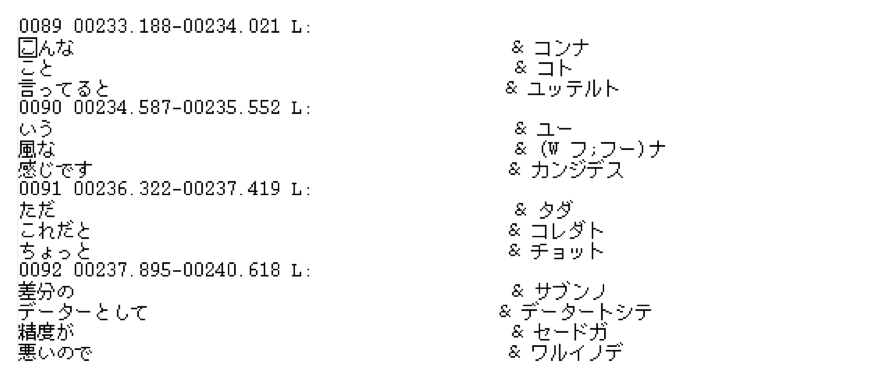
\includegraphics{./figure/kakiokosi.eps}
  \end{center}
  \caption{書き起こしテキストの例 \label{fig:kakiokosi}}
\end{figure}

本研究ではこのCSJをベースに学習テキストを構成する。使用するデータは977講演分のテキストで、約14MBである。

\vspace{0.2in}\noindent{\textbf{\underline{拡張したコーパスによる学習テキスト}}}\par
この学習テキストは江頭らによる、学術講演の書き起こしと新聞記事に拡張されるテキストとして参加者名の入ったテキスト、Webから収集してきたテキスト、そして対話コーパスから作成される対話テキストを追加した未知語の減少に着目した学習テキストである。この学習テキストは会議中に参加者の名前を呼ぶことが多い、会議は対話形式であるなどの会議の特徴を考慮した学習テキストである。テキストサイズは約100MBである。以降本論文では、このテキストを拡張したコーパスによる学習テキストと呼ぶ。

\vspace{0.2in}\noindent{\textbf{\underline{拡張したコーパスによる学習テキスト}}}\par
この学習テキストは荒井らによる、会議における発話行為に着目して作成された学習テキストである。学術講演の書き起こしと新聞記事に対話表現に近い特徴を持っていると考えられるQ&Aサイトから収集したテキストと対話コーパスを追加した学習テキストである。テキストサイズは約44MBである。以降本論文ではこのテキストを対話特化テキストと呼ぶ。


\subsection{評価方法}
本研究では評価尺度としては式\ref{calc:word_acc}で与えられる単語正解精度$Acc$(Word Accuracy)を用いる。ここで$W$は単語数、$S$(Substitution)は置換誤り、$D$(Deletion)は脱落誤り、$I$(Insertions)は挿入誤りの単語数を表わす。置換誤りとは、正解の単語が別の単語に誤認識された場合の誤りである。脱落誤りとは、単語があるべき部分に認識結果が何も出力されなかった場合の誤りである。挿入誤りは、本来単語がない部分に誤認識結果として単語が出力された場合の誤りである。

\begin{equation}
\label{calc:word_acc}
Acc=\frac{(W-S-D-I)}{W}
\end{equation}

          
評価は、正解ファイルと認識結果のファイルをDPマッチングを行なうことにより算出する。この正解ファイルは形態素解析した結果の形態素列によって作成したものである。
また、本研究ではアンカーの発話区間を対象とした音声認識を行うため、\ref{chapter:get_anchor}章で検出した発話区間より、アンカー以外の発話区間で認識された単語は全て挿入誤り、アンカーの発話として検出出来なかった発話区間の単語は全て削除誤りとして計算する。
\subsection{実験結果}
\subsection{考察}
  % 音声認識実験

\section{アンカーの発話群検出実験}
本節では、i-vectorを用いてアンカーの発話区間検出を行う。
\label{chapter:get_anchor}
\subsection{実験方法}
本節では、\ref{chapter:connect_sp}節の手法1で得られたi-vectorを用いてアンカーの発話区間検出を行う。i-vectorを用いたアンカーの発話区間抽出方法を\ref{section:clustering}節に示す。

\subsection{評価方法}
評価は、検出されたアンカーの発話区間と正解ラベルを比較して行う。

\begin{table}[H]
\begin{center}
    \caption{アンカーの発話区間の正誤判定 \label{table:clustering}}
\begin{tabular}{|c|c|c|c|l}
\cline{1-4}
\multicolumn{2}{|c|}{\multirow{2}{*}{}} & \multicolumn{2}{c|}{「発話者」のラベルが付与された発話区間} &  \\ \cline{3-4}
\multicolumn{2}{|c|}{}                  & アンカーの発話区間        & アンカー以外の発話区間        &  \\ \cline{1-4}
\multirow{2}{*}{判定結果}        & 正        & $TP$                  & $FP$                   &  \\ \cline{2-4}
& 誤        & $FN$                  & $TN$                   &  \\ \cline{1-4}
\end{tabular}
\end{center}
\end{table}

表\ref{table:clustering}を用いて、$P$(適合率(Precision))と$R$(再現率(Recall))を式\ref{calc:precision2}と式\ref{calc:recall2}のようにそれぞれ定義する。また、$F$値($F-measure$)を式\ref{calc:fmeasure2}のように定義する。

\begin{equation}
\label{calc:precision2}
P = \frac{TP}{TP + FP}
\end{equation}

\begin{equation}
\label{calc:recall2}
R = \frac{TP}{TP + FN}
\end{equation}

\begin{equation}
\label{calc:fmeasure2}
F = \frac{1}{\frac{1}{P} + \frac{1}{R}}
\end{equation}

ここで$P$と$R$はそれぞれ適合率、再現率を表す。

また、検出したアンカーの発話区間の割合を式\ref{calc:anchor_acc}のように定義して評価する。

\begin{equation}
\label{calc:anchor_acc}
Acc_{time} = \frac{検出したアンカーの発話区間の時間数}{アンカーの発話区間の時間数}
\end{equation}

本実験では、評価方法として適合率、再現率、$F$値、$Acc_{time}$を用いる。

\subsection{実験結果}
アンカーの発話区間検出精度を以下に示す。

\begin{table}[H]
  \begin{center}
    \caption{アンカーの発話区間検出精度($Th_{time}=0.8)$ \label{table:result_get_anchor08}}
    \begin{tabular}{|c||c|c|c|c|} \hline
      $Th_{cos}$ & $Recall$ & $Precision$ & $F-measure$ & $Acc_{time}$\\ \hline
0.5 & 0.836 & 0.632 & 0.72 & 0.794 \\ \hline
0.6 & 0.812 & 0.768 & 0.789 & 0.774 \\ \hline
0.7 & 0.778 & 0.866 & 0.82 & 0.747 \\ \hline
0.8 & 0.656 & 0.92 & 0.766 & 0.655 \\ \hline

    \end{tabular}
  \end{center}
\end{table}

\begin{table}[H]
  \begin{center}
    \caption{アンカーの発話区間検出精度($Th_{time}=0.9$) \label{table:result_get_anchor09}}
    \begin{tabular}{|c||c|c|c|c|} \hline
      $Th_{cos}$ & $Recall$ & $Precision$ & $F-measure$ & $Acc_{time}$\\ \hline
0.5 & 0.839 & 0.636 & 0.723 & 0.794 \\ \hline
0.6 & 0.81 & 0.775 & 0.792 & 0.771 \\ \hline
0.7 & 0.782 & 0.865 & 0.821 & 0.747 \\ \hline
0.8 & 0.681 & 0.915 & 0.781 & 0.671 \\ \hline

    \end{tabular}
  \end{center}
\end{table}

\begin{table}[H]
  \begin{center}
    \caption{アンカーの発話区間検出精度($Th_{time}=1.0$) \label{table:result_get_anchor10}}
    \begin{tabular}{|c||c|c|c|c|} \hline
      $Th_{cos}$ & $Recall$ & $Precision$ & $F-measure$ & $Acc_{time}$\\ \hline
0.5 & 0.837 & 0.638 & 0.724 & 0.793 \\ \hline
0.6 & 0.811 & 0.764 & 0.787 & 0.768 \\ \hline
0.7 & 0.784 & 0.867 & 0.824 & 0.747 \\ \hline
0.8 & 0.683 & 0.912 & 0.781 & 0.668 \\ \hline

    \end{tabular}
  \end{center}
\end{table}

\begin{table}[H]
  \begin{center}
    \caption{アンカーの発話区間検出精度($Th_{time}=1.1$) \label{table:result_get_anchor11}}
    \begin{tabular}{|c||c|c|c|c|} \hline
      $Th_{cos}$ & $Recall$ & $Precision$ & $F-measure$ & $Acc_{time}$\\ \hline
0.5 & 0.84 & 0.609 & 0.706 & 0.793 \\ \hline
0.6 & 0.815 & 0.714 & 0.761 & 0.772 \\ \hline
0.7 & 0.773 & 0.871 & 0.819 & 0.74 \\ \hline
0.8 & 0.688 & 0.91 & 0.783 & 0.675 \\ \hline

    \end{tabular}
  \end{center}
\end{table}


\begin{table}[H]
  \begin{center}
    \caption{アンカーの発話区間検出精度($Th_{time}=1.2$) \label{table:result_get_anchor12}}
    \begin{tabular}{|c||c|c|c|c|} \hline
      $Th_{cos}$ & $Recall$ & $Precision$ & $F-measure$ & $Acc_{time}$\\ \hline
0.5 & 0.841 & 0.587 & 0.692 & 0.793 \\ \hline
0.6 & 0.811 & 0.734 & 0.771 & 0.768 \\ \hline
0.7 & 0.774 & 0.877 & 0.822 & 0.741 \\ \hline
0.8 & 0.687 & 0.907 & 0.782 & 0.673 \\ \hline

    \end{tabular}
  \end{center}
\end{table}

\begin{table}[H]
  \begin{center}
    \caption{アンカーの発話区間検出精度($Th_{time}=1.3$) \label{table:result_get_anchor13}}
    \begin{tabular}{|c||c|c|c|c|} \hline
      $Th_{cos}$ & $Recall$ & $Precision$ & $F-measure$ & $Acc_{time}$\\ \hline
0.5 & 0.841 & 0.589 & 0.693 & 0.793 \\ \hline
0.6 & 0.809 & 0.699 & 0.75 & 0.769 \\ \hline
0.7 & 0.776 & 0.868 & 0.819 & 0.741 \\ \hline
0.8 & 0.686 & 0.902 & 0.779 & 0.672 \\ \hline

    \end{tabular}
  \end{center}
\end{table}

\begin{table}[H]
  \begin{center}
    \caption{アンカーの発話区間検出精度($Th_{time}=1.4$) \label{table:result_get_anchor14}}
    \begin{tabular}{|c||c|c|c|c|} \hline
      $Th_{cos}$ & $Recall$ & $Precision$ & $F-measure$ & $Acc_{time}$\\ \hline


    \end{tabular}
  \end{center}
\end{table}

\begin{table}[H]
  \begin{center}
    \caption{アンカーの発話区間検出精度($Th_{time}=1.5$) \label{table:result_get_anchor15}}
    \begin{tabular}{|c||c|c|c|c|} \hline
      $Th_{cos}$ & $Recall$ & $Precision$ & $F-measure$ & $Acc_{time}$\\ \hline


    \end{tabular}
  \end{center}
\end{table}
\subsection{考察}

\chapter{結論}
本稿では、ニュース番組音声のインデクス自動付与に向けたダイアライゼーション実現のために、発話間隔と発話環境を考慮したi-vectorを用いたニュースアンカーの発話検出精度向上を目指した。\par
特定話者の識別にはi-vectorが一般的に用いられるが、短い発話からは話者の識別に必要な十分な話者の特徴を抽出できない。そのため、本稿では前後の発話区間が同一話者の発話である可能性が高いとき発話区間を結合し、長い発話を擬似的に作成した。次に、結合した発話区間からi-vectorを抽出することで短い発話から得られるi-vectorの抽出精度向上を目指した。発話区間の結合には、同一話者が連続で発話する場合間をおかずに発話すること、話者が切り替わった時に発話環境が変化することに着目し、発話と発話の時間間隔を考慮する手法と、発話者の発話環境を考慮する手法を用いた。以上の手法を用いて結合した発話区間から抽出したi-vectorを用いてニュースアンカーの発話検出を行った結果、発話検出精度が約6\%向上し、ニュースアンカーの発話検出への有意性を示した。また、本研究で抽出したi-vectorを用いてニュースアンカーの音声認識を行なった。音声認識はニュースアンカーの発話区間が既知の場合と未知の場合で行い、発話区間が既知のときは音声認識精度の向上が確認できなかった。しかし、ニュースアンカーの発話区間が未知の場合、従来と比較してニュースアンカーの発話区間検出精度が向上したことが音声認識精度の向上に繋がった。\par
今後の課題として、ニュース音声の背景雑音の除去が挙げられる。ニュースアンカーはスタジオで発話しているため基本的には雑音が入らないが、参考映像などの音が発話中に流れることがある。そのため、雑音、音楽に対して音源分離などの処理をすることでi-vectorの抽出精度をはじめ、アンカーの発話区間検出精度、音声認識精度が向上すると考えられる。
  % まとめ

\appendix
%\chapter*{付録}

%\section{コサイン類似度を用いたi-vectorの性質の調査}
\label{section:pre_cos}
\subsection{使用する音声データ}
\label{section:detail_ATR}
UBMモデルの学習データおよびコサイン類似度を用いたi-vectorの性質の調査に読み上げ音声\cite{ATR}を使用した。読み上げ音声には、男女各110人$×$50発話分が収録されている。

\subsection{調査方法}
各話者の音声データから1つの発話を取り出し、それ以外の音声データとのi-vectorのコサイン類似度を算出する。また、同一話者の発話間の場合と異なる話者の発話間の2つの場合で発話の長さごとのコサイン類似度が取る値の検証を行う。\par

\subsection{コサイン類似度の算出条件}
i-vectorの抽出には、ALIZEとLIR RAL\cite{alize}を用いる。読み上げ音声に収録されている各発話データからi-vectorを抽出する。発話データから抽出する音響特徴パラメータを表\ref{iv_feature}に示す。また混合数は32とした。

\begin{table}[H]
  \begin{center}
    \caption{使用する音響特徴パラメータ}
    \label{iv_feature}
    \begin{tabular}{|c||c|} \hline
      特徴量 & 次元数\\ \hline
      MFCC & 19  \\ 
      POW & 1  \\ 
      $\Delta$MFCC & 19 \\ 
      $\Delta$POW & 1 \\ 
      $\Delta\Delta$MFCC & 19 \\ 
      $\Delta\Delta$POW & 1 \\ \hline
      計 & 60 \\ \hline
    \end{tabular}
  \end{center}
\end{table}

本稿では、音響特徴量のひとつとしてメル周波数ケプストラム係数(MFCC)を用いる。メル周波数ケプストラム係数(Mel - Frequency Cepstrum Coefficient : MFCC)とは、メル周波数という人間の音の高低に対する感覚尺度を考慮した特徴量であり、音声スペクトルから係数スペクトルを抽出したものである。これは一般的に、音声の特徴を抽出するパラメータとして用いられる。[5]

\subsection{調査結果}
\noindent{\textbf{\underline{同一話者間のi-vectorの特徴}}}\par
同一話者間のi-vectorのコサイン類似度を図\ref{fig:same_cos_hist}、その標準偏差を図\ref{fig:same_cos_vari}に示す。\par

\begin{figure}[H]
  \begin{center}
    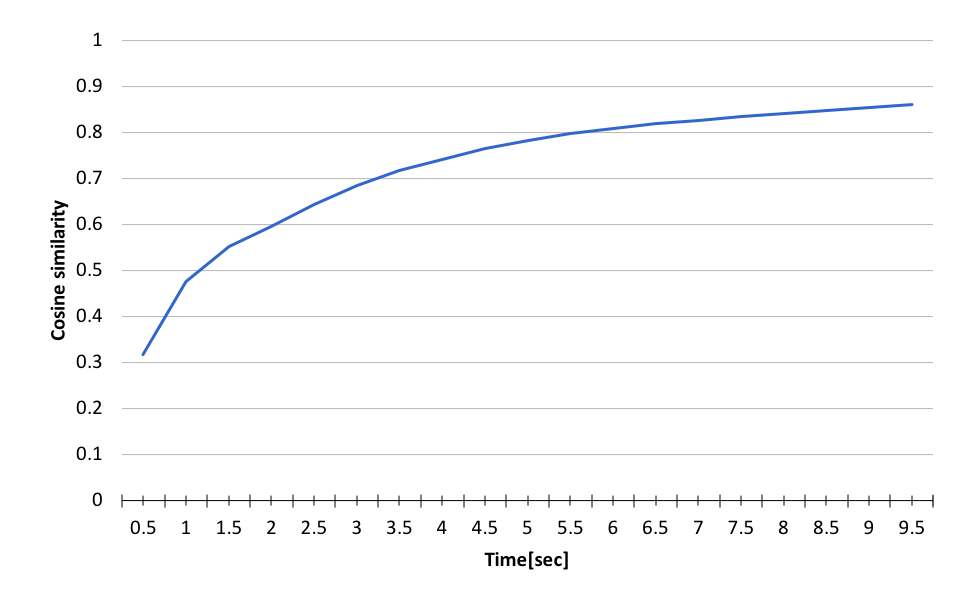
\includegraphics[scale=0.8]{./figure/same_cos_hist.eps}
  \end{center}
  \caption{同一話者間のi-vectorのコサイン類似度 \label{fig:same_cos_hist}}
\end{figure}

\begin{figure}[H]
  \begin{center}
    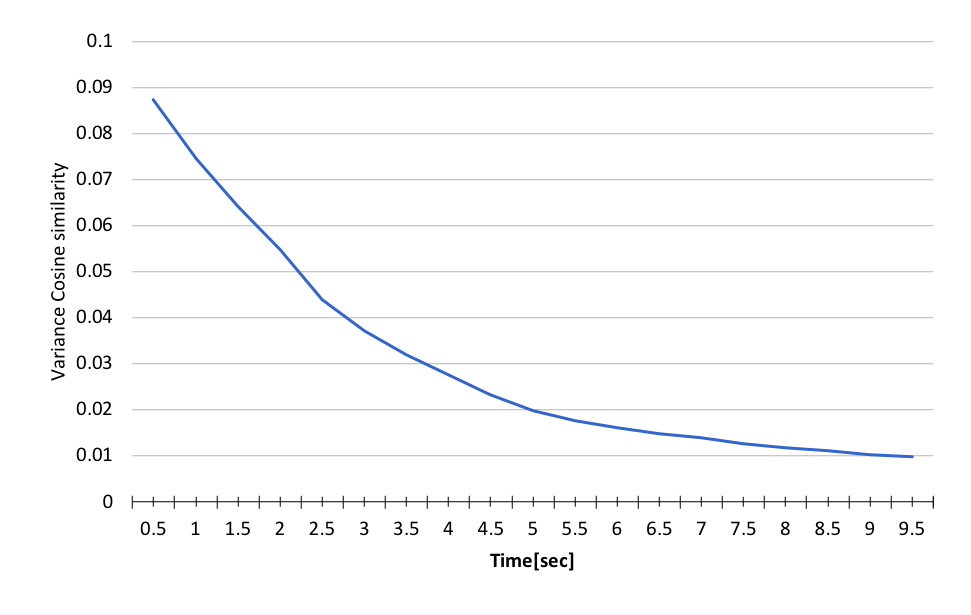
\includegraphics[scale=0.8]{./figure/same_cos_vari.eps}
  \end{center}
  \caption{同一話者間のi-vectorのコサイン類似度の標準偏差 \label{fig:same_cos_vari}}
\end{figure}

図\ref{fig:same_cos_hist}より、発話が長いほどコサイン類似度の値が高くなる傾向にある。また、図\ref{fig:same_cos_vari}より、発話が短い場合はコサイン類似度のばらつきが大きく、長くなるにつれて収束する傾向にある。\par


\vspace{0.2in}\noindent{\textbf{\underline{異なる話者間のi-vectorの特徴}}}\par
異なる話者間のi-vectorのコサイン類似度を図\ref{fig:other_cos_hist}、その標準偏差を図\ref{fig:other_cos_vari}に示す。\par

\begin{figure}[H]
  \begin{center}
    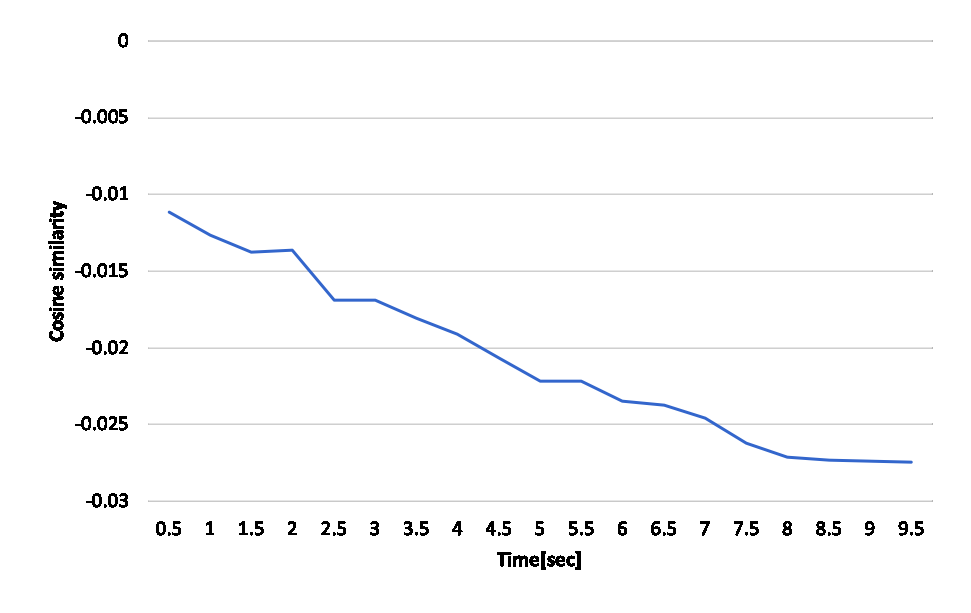
\includegraphics[scale=0.8]{./figure/other_cos_hist.eps}
  \end{center}
  \caption{異なる話者間のi-vectorのコサイン類似度 \label{fig:other_cos_hist}}
\end{figure}

\begin{figure}[H]
  \begin{center}
    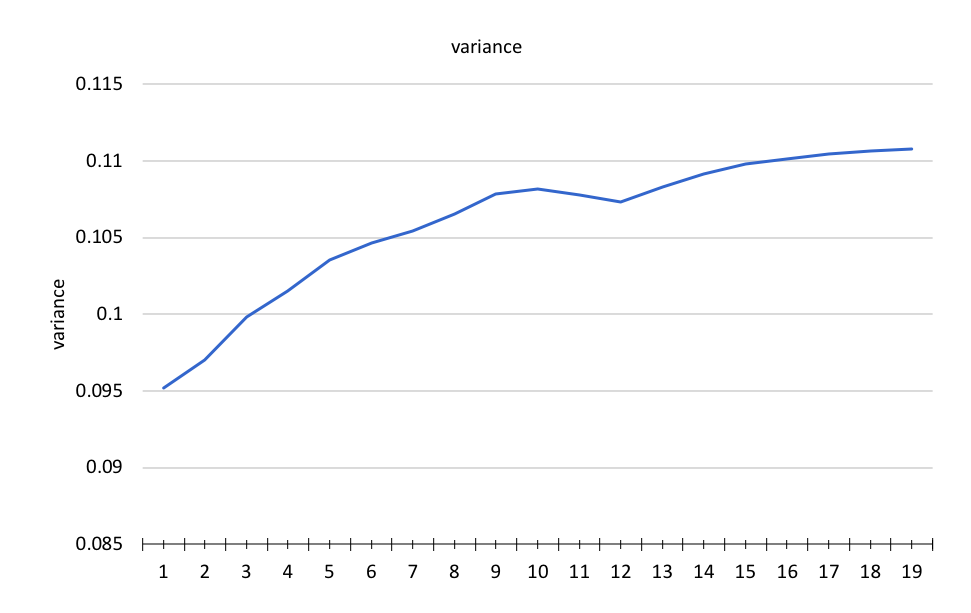
\includegraphics[scale=0.8]{./figure/other_cos_vari.eps}
  \end{center}
  \caption{異なる話者間のi-vectorのコサイン類似度の標準偏差 \label{fig:other_cos_vari}}
\end{figure}

図\ref{fig:other_cos_hist}より、発話が長くなるほどコサイン類似度が低くなる傾向にある。また、図\ref{fig:other_cos_vari}より、発話が長くなるごとにコサイン類似度のばらつきが大きくなる傾向にある。\par

\subsection{考察}
発話が短い時、同一話者間のコサイン類似度のばらつきが大きい理由として、短い発話からは話者の特徴が十分に抽出できていないためであると考えられる。また発話が短い時、異なる話者間のコサイン類似度のばらつきが小さいことから、話者の特徴を抽出できていない場合、話者が異なっていてもi-vectorのコサイン類似度が似た値をとることがわかる。つまり、i-vectorを用いた話者識別、話者照合を行う場合、できるだけ長い発話を用いる必要がある。

\chapter{音源分離実験}
\label{section:devide_audio}
\renewcommand{\labelenumi}{(\arabic{enumi})}
音響データ(ニュース音声、会話音声等)の中にはさまざまな音源種別(声、音楽、雑音等)の音が混在している。音源識別とは、音響データ中に含まれる音源種別を自動的に識別することである。ここでの処理は、音響データのスペクトル解析を行い、音響特徴パラメータを求め、あらかじめ用意した各音源種別の音響特徴パラメータの分布と比較することで音源種別を識別する。\par
本研究では、ニュース番組の音声データに音響特徴パラメータを用いた音源識別\cite{shimae_9} を用い、音声データ中の音源種別を以下の4つに分類した。

\begin{enumerate}
\item 音声区間: アナウンサーやインタビューの声
\item 音楽区間: オープニングやエンディングなどの音楽、BGM
\item 背景雑音区間: 自動車走行音や鳥の泣き声
\item 無音区間: 音量が極めて小さい区間
\end{enumerate}\par

また、音源識別システムは音響データを各種別へ識別するための音響特徴パラメータの分布に混合ガウス分布を用いている。本研究では、混合数8のガウス分布を使用している。本研究の音響特徴パラメータを表2.2、各音源種別の識別性能F 値を表\ref{ad_F} に示す。ただし、表の評価値とは、音源種別間のデータ数を考慮するために、各音源種別のF 値に各音源種別の割合をかけ、合計したものである。\par

表2.2: 音源識別のための音響特徴パラメータ

\begin{table}[htb]
  \begin{center}
    \caption{音源識別システムのF値}
    \label{ad_F}
    \begin{tabular}{|c||c|} \hline
       & F値$[\%]$\\ \hline
      Speech & 94.84  \\ \hline
      Music & 83.32 \\ \hline
      Noise & 63.73  \\ \hline
      Pause & 77.43 \\ \hline
      評価値 & 87.19 \\ \hline
    \end{tabular}
  \end{center}
\end{table}



以下に、音源識別のためのスペクトル解析と音響特徴パラメータについて説明する。\par


\subsection{スペクトル解析}
音響データのスペクトル解析の手法として最も一般的に利用されている方法は、短時間フーリエスペクトル分析がある。この方法は、音響データから連続する数10ms 程度の時間長の信号区間を切り出し、切り出された信号が定常性(一定周期で繰り返す)と仮定して、スペクトル解析を行う。\par
スペクトル解析の流れは以下の通りである。

\begin{enumerate}
\item フレーム化処理:与えられた信号$s(n)$ に長さ$N$ の分析窓を掛けることで以下のような信号系列$s_\omega(m; l)$を取り出す。
\begin{equation}
S_w(m;l)=\sum_{m=0}^{N-1}\omega(m)s(l+m)\qquad(l=0,T,2T,\cdots)
\end{equation}

ここで、添え字$l$は信号の切り出し位置に対応している。すなわち、$l$を一定間隔$T$で増加させることで定常とみなされる長さ$N$の信号系列$s_\omega(n)\quad (n=0,1,\cdots,N-1)$が間隔$T$で得られる。この処理をフレーム化処理と呼び、$N$をフレーム長、$T$をフレーム間隔と呼ぶ。

\item 窓関数をかける:ある有限区間以外で0となる関数であり、フレーム化されたデータに対して重みをつける関数である。フレーム化処理を行う場合、離散的なデータの繋ぎ目においての信号の急激な変化の影響を和らげるため、原則として窓関数をかけなければならない。代表的なものとして音声信号だけに有効なハニング窓と、音声信号以外にも様々な信号にも有効なハミング窓がある。

\begin{equation}
\label{da1}
ハニング窓:\omega(n)=0.5-0.5\cos(\frac{2\pi n}{N-1})\qquad(n=0,1,\cdots,N-1)
\end{equation}

\begin{equation}
\label{da2}
ハミング窓:\omega(n)=0.54-0.54\cos(\frac{2\pi n}{N-1})\qquad(n=0,1,\cdots,N-1)
\end{equation}

\item スペクトル分析(離散時間フーリエ変換、高速フーリエ変換):フレーム化処理によって得られた信号系列の短時間フーリエスペクトルは、離散時間フーリエ変換により以下の式で与えられる。
\begin{equation}
S(n)=\sum s_\omega(n)e^{-j2\pi \frac{nk}{N}} \qquad (k=0,1,\cdots,N-1)
\end{equation}

離散フーリエ変換(DFT) は、離散的なデータをフーリエ変換する際に、通常のフーリエ変換の無限区間積分を有限の和で書き換えたもので、時間領域、周波数領域ともに離散化されたフーリエ変換のことであり、時間領域の表現を周波数領域における表現に変換する。また、逆に周波数領域の表現を時間領域の表現に変換する、つまり元の音響データに戻す変換を離散フーリエ逆変換(IDFT) と呼び以下の式で与えられる。

\begin{equation}
S(n)=\frac{1}{N}\sum S(k)e^{j2\pi \frac{nk}{N}} \qquad (k=0,1,\cdots,N-1)
\end{equation}

実際の信号処理過程では、離散的フーリエ変換(DFT) をその高速算法である高速フーリエ変換(FFT) を用いて実行し、当該音声区間のスペクトル表現とすることが一般的である。高速フーリエ変換は式(\ref{da1})、(\ref{da2}) の$N$ が$2^n$ 個であるとき、その処理を高速にできる性質がある。フーリエ変換の式には、

\begin{equation}
S\prime(n)=S(e^{j\frac{2\pi}{n}k})=\sum s_\omega(n)e^{-j2\pi \frac{2\pi}{N}kn} \qquad (k=0,1,\cdots,N-1)
\end{equation}

なる複素系列$S\prime(k)$が音声スペクトル表現として最も一般的に用いられる。

\item パワースペクトルの算出:音響信号の特徴は主として、調音フィルタの振幅伝達特性に含まれる。したがって、音響信号の振幅スペクトル$|S^\prime(k)|$、あるいはその2 乗のパワースペクトル$|S^\prime(k)|^2$、対数スペクトル$10\log|S^\prime(k)|^2$が注目すべきスペクトル表現になる。このスペクトルをグラフにすることで、音響データに含まれている周波数成分を解析することができる。音響データに含まれている周波数成分の上限はサンプリング定理により、サンプリング周波数の半分なので、高速フーリエ変換における周波数成分が意味のあるスペクトルとして扱われるのは0 から$\pi$までのスペクトルである。また、音響信号の離散パワースペクトル系列は、離散スペクトル系列から式(\ref{da3}) で表される。

\begin{equation}
\label{da3}
|S^\prime(k)|^2=\frac{1}{N}[\operatorname{Re}\left\{S^\prime(k)\right\}^2+\operatorname{Im}\left\{S^\prime(k)\right\}^2]
\end{equation}

この2 乗値のパワースペクトル$|S^\prime(k)|^2$を特徴量として扱っている。音響信号に高速フーリエ変換を施すと、時間表現(縦軸:パワー、横軸:時間) から周波数表現(縦軸:振幅、横軸:周波数) へと変換できる。しかし、実際には縦軸を周波数、横軸を時間としたグラフがよく使用されており、このようなグラフをスペクトルグラムという。スペクトルグラムは音声を視覚化したものであり、声紋とも呼ばれる。

\end{enumerate}\par
\subsection{音響特徴パラメータ}
本研究で使用する7つの音響特徴パラメータについて述べる\cite{shimae_10}

\begin{enumerate}
\item スペクトルの変化\par
動的特徴量を連続するスペクトルのフレーム間の変化量として取り出す。音響信号のスペクトル分析した連続するフレームにおいて、あるフレームとその一定時間後のフレームとのパワースペクトルの差分によりスペクトルの変化量を得て、そのスペクトルの差分を一定時間足し合わせたものとしている。スペクトルの変化量によって比較する利点は、音声の識別に有利であり音声に比べて背景雑音のほうがスペクトルの変化量が大きく、無音のほうがスペクトルの変化量が小さいということである。

\item スペクトルの傾き\par
あらかじめ人手により作成したラベルにより音響データの各区間を各種別(音声、音楽、背景雑音、無音)に振り分け、それぞれに対してスペクトル分析を行い、パワースペクトルを取り出し、各種別内において集められたパワースペクトルの分布を求めることで各種別において傾き値を得る。この傾き値を基に、与えられた音響ファイルから次々に得るパワースペクトルと各種別の学習データとの特徴パラメータの分布の類似度を比較する。この最小単純形は、パワースペクトルにおける一次回帰直線の傾きを比べることと同じである。傾きによって比較する利点は、有色系の音のほうが白色雑音よりも傾きが大きいので、音声と音楽と無音の識別に有利である。

\item 白色雑音との近さ\par
パワースペクトルより一次回帰直線からスペクトル波形の切片を求めることで入力信号の白色性の度合を計測する。この白色雑音との近さによって比較する利点は、背景雑音のような定常的に混入した雑音は白色性が高いので、これらの識別ができるこということである。

\item ピッチ\par
有声音源の繰り返し周期、いわゆるピッチ(基本周波数)の変化を調べることで、音源の変化を知ることができ、音源の特定のパラメータである。周波数分析によりピッチを求め、学習データと比べることで音源の特定に用いる。

\item パワー\par
時間領域の分析だが、音響信号のような非定常的な信号に対して、変化していく信号の大きさにうまく追随するような比較的短い区間に音響データを区切り、その区間の信号$xl(n)$に対してエネルギー$E(l)$ を定義する\cite{shimae_11}。
\begin{equation}
E(l)=\sum_{n=0}^{N-1}\left\{x_l(n)\right\}^2
\end{equation}
ここでは、整数$N$ は窓の中に含まれる音響信号の数である。\par
利点としては、測定が簡単であり、音声認識における有色系の音の区間の抽出にもよく用いられることから、有音と無音の区別に有利である。

\item 中心周波数\par
抽出したパワースペクトルにおいて、無音の場合は右下がりに傾斜しているが、有音の場合は傾斜の途中で膨らみまたは突起が発生する。その突起がもっとも大きく発生している周波数帯の中心部分の周波数を中心周波数として定義している。これは有音と無音の識別に効果がある。

\item 中心周波数のバンド幅\par
中心周波数を含む膨らみ、あるいは突起の始まりと終わりによる周波数帯の長さをバンド幅として定義する。音声は一定の周波数を含むことが多いためそのバンド幅はある程度の大きさになることが考えられるが、雑音はあまり多くの周波数を含まないものから白色性が高く幅広い周波数を含むものまで様々であり、その違いから音声と雑音の特定に有効である。
\end{enumerate}\par

\section{使用する音声データ}
\label{section:detail_train_news}
本調査では、ニュース番組の音声データ12個を用いる。各音声データには、事前に人手で3種類(音楽、音声、雑音)の音源ラベルが付与されている。「音声」の音源ラベルが付与された区間においては、更に発話者の情報が付与されている。表\ref{fig:example_label}は音声の音源ラベルの一例である。また「音声」の音源ラベルをもとに対象の音声データから発話区間を抽出し、それを一発話とした。表\ref{table:train_detail}に調査に用いるデータの詳細を示す。\vspace{0.2in}

\section{調査方法}
\ref{section:devide_audio}節で述べた音源分離を用いての音源分離を行う。
表\ref{table:detail_identification_method1}は音源識別の調査条件である。

\begin{table}[H]
  \begin{center}
    \caption{音源識別実験の実験条件 \label{table:detail_identification_method1}}
    \begin{tabular}{|c||c|} \hline
      FFTの窓幅(フレーム長) & 2048point(約0.046[sec])   \\ \hline
      FFTのシフト幅(フレーム間隔) &  1024point(約0.023[sec]) \\ \hline
      窓関数 & ハミング窓  \\ \hline
    \end{tabular}
  \end{center}
\end{table}

また、検出する区間は「音声」「背景雑音」「音楽」「無音」の4つである。

\subsection{評価方法}
評価は、検出された各区間と正解ラベルを比較して行う。

\begin{table}[H]
\begin{center}
    \caption{検出した区間の正誤判定 \label{table:search_table}}
\begin{tabular}{|c|c|c|c|l}
\cline{1-4}
\multicolumn{2}{|c|}{\multirow{2}{*}{}} & \multicolumn{2}{c|}{正解ラベル} &  \\ \cline{3-4}
\multicolumn{2}{|c|}{}                  & ラベルが付与された区間        &    ラベルが付与されていない区間     &  \\ \cline{1-4}
\multirow{2}{*}{判定結果}        & 正        & $TP$                  & $FP$                   &  \\ \cline{2-4}
& 誤        & $FN$                  & $TN$                   &  \\ \cline{1-4}
\end{tabular}
\end{center}
\end{table}

表\ref{table:search_table}が得られると$P$(適合率(Precision))と$R$(再現率(Recall))は式\ref{calc:precision}と式\ref{calc:recall}のようにそれぞれ定義できる。

\begin{equation}
\label{calc:precision}
P = \frac{TP}{TP + FP}
\end{equation}

\begin{equation}
\label{calc:recall}
R = \frac{TP}{TP + FN}
\end{equation}

適合率が高い値を取るとき、識別結果に含まれる「誤り」の割合が少ないことを示している。また再現率が高いとき、識別結果に「漏れ」が少ないことを示している。一般的に、再現率の高いシステムは適合率が低く、逆に適合率が高いシステムは再現率が低い傾向にある。評価指標が2つあるとどちらのシステムが優れているかの判断が難しいため、適合率と再現率の調和平均を取り、ひとつのスカラ値に変換したF値(F-measure)がある。

\begin{equation}
\label{calc:fmeasure}
F = \frac{2 \times P \times R}{P + R}
\end{equation}

ここで$P$と$R$はそれぞれ適合率、再現率を表す。\par
本調査では、評価指標として適合率、再現率、F値を用いる。

\subsection{調査結果}
表\ref{table:NHK_speach_RPF} $\sim$ 表\ref{table:NHK_pause_RPF}に音源識別による識別精度を示す。
\begin{table}[H]
  \begin{center}
    \caption{発話区間検出精度 \label{table:NHK_speach_RPF}}
    \begin{tabular}{|c||c|c|c|} \hline
データID & Recall & Precision & F-meature \\ \hline
ニュースA & 0.892 & 0.966 & 0.928 \\ \hline
ニュースB & 0.888 & 0.963 & 0.924 \\ \hline
ニュースC & 0.883 & 0.963 & 0.921 \\ \hline
ニュースD & 0.902 & 0.952 & 0.927 \\ \hline
ニュースE & 0.884 & 0.970 & 0.925 \\ \hline
ニュースF & 0.907 & 0.974 & 0.939 \\ \hline
ニュースG & 0.907 & 0.961 & 0.933 \\ \hline
ニュースH & 0.843 & 0.966 & 0.900 \\ \hline
ニュースI & 0.886 & 0.982 & 0.932 \\ \hline
ニュースJ & 0.902 & 0.980 & 0.939 \\ \hline
ニュースK & 0.875 & 0.963 & 0.917 \\ \hline
ニュースL & 0.886 & 0.963 & 0.923 \\ \hline
 平均 & 0.888 & 0.967 & 0.926 \\ \hline
    \end{tabular}
  \end{center}
\end{table}

\begin{table}[H]
  \begin{center}
    \caption{音楽区間検出精度 \label{table:NHK_music_RPF}}
    \begin{tabular}{|c||c|c|c|} \hline
データID & Recall & Precision & F-meature \\ \hline
ニュースA & 0.467 & 0.565 & 0.511 \\ \hline
ニュースB & 0.508 & 0.640 & 0.566 \\ \hline
ニュースC & 0.507 & 0.687 & 0.583 \\ \hline
ニュースD & 0.429 & 0.661 & 0.520 \\ \hline
ニュースE & 0.481 & 0.633 & 0.547 \\ \hline
ニュースF & 0.627 & 0.699 & 0.661 \\ \hline
ニュースG & 0.611 & 0.936 & 0.740 \\ \hline
ニュースH & 0.570 & 0.406 & 0.474 \\ \hline
ニュースI & 0.481 & 0.648 & 0.552 \\ \hline
ニュースJ & 0.531 & 0.776 & 0.631 \\ \hline
ニュースK & 0.718 & 0.381 & 0.498 \\ \hline
ニュースL & 0.672 & 0.471 & 0.554 \\ \hline
 平均 & 0.537 & 0.622 & 0.576 \\ \hline
    \end{tabular}
  \end{center}
\end{table}

\begin{table}[H]
  \begin{center}
    \caption{背景雑音区間検出精度 \label{table:NHK_noise_RPF}}
    \begin{tabular}{|c||c|c|c|} \hline
データID & Recall & Precision & F-meature \\ \hline
ニュースA & 0.259 & 0.835 & 0.395 \\ \hline
ニュースB & 0.406 & 0.681 & 0.509 \\ \hline
ニュースC & 0.199 & 0.857 & 0.323 \\ \hline
ニュースD & 0.225 & 0.678 & 0.338 \\ \hline
ニュースE & 0.282 & 0.783 & 0.414 \\ \hline
ニュースF & 0.145 & 0.587 & 0.233 \\ \hline
ニュースG & 0.192 & 0.855 & 0.313 \\ \hline
ニュースH & 0.235 & 0.803 & 0.364 \\ \hline
ニュースI & 0.338 & 0.817 & 0.478 \\ \hline
ニュースJ & 0.268 & 0.746 & 0.395 \\ \hline
ニュースK & 0.268 & 0.906 & 0.413 \\ \hline
ニュースL & 0.349 & 0.511 & 0.415 \\ \hline
 平均 & 0.263 & 0.756 & 0.390 \\ \hline
    \end{tabular}
  \end{center}
\end{table}

\begin{table}[H]
  \begin{center}
    \caption{無音区間検出精度 \label{table:NHK_pause_RPF}}
    \begin{tabular}{|c||c|c|c|} \hline
データID & Recall & Precision & F-meature \\ \hline
ニュースA & 0.883 & 0.659 & 0.755 \\ \hline
ニュースB & 0.334 & 0.685 & 0.449 \\ \hline
ニュースC & 0.923 & 0.669 & 0.776 \\ \hline
ニュースD & 0.581 & 0.587 & 0.584 \\ \hline
ニュースE & 0.807 & 0.693 & 0.745 \\ \hline
ニュースF & 0.859 & 0.564 & 0.681 \\ \hline
ニュースG & 0.934 & 0.659 & 0.773 \\ \hline
ニュースH & 0.788 & 0.626 & 0.698 \\ \hline
ニュースI & 0.907 & 0.708 & 0.795 \\ \hline
ニュースJ & 0.763 & 0.645 & 0.699 \\ \hline
ニュースK & 0.887 & 0.615 & 0.726 \\ \hline
ニュースL & 0.602 & 0.702 & 0.648 \\ \hline
 平均 & 0.787 & 0.649 & 0.712 \\ \hline
    \end{tabular}
  \end{center}
\end{table}

\begin{table}[H]
  \begin{center}
    \caption{発話区間検出精度 \label{table:test_detail_RPF}}
    \begin{tabular}{|c||c|c|c|} \hline
      データID & Recall & Precision & F-meature \\ \hline
      ニュース1 & 0.895 & 0.916 & 0.905 \\ \hline
      ニュース2 & 0.841 & 0.955 & 0.895\\ \hline
      ニュース3 & 0.883 & 0.860 & 0.871 \\ \hline
      ニュース4 & 0.901 & 0.833 & 0.866\\ \hline
      ニュース5 & 0.910 & 0.930 & 0.906\\ \hline
    \end{tabular}
  \end{center}
\end{table}

音声区間の検出精度は高い精度を示した。背景雑音の区間はRecallが非常に低いがPrecisionが非常に高い結果となった。
また、ニュース番組によって発話区間の検出精度に差が生じた。

\section{考察}
背景雑音区間と音楽区間の検出精度が音声区間と無音区間の区間検出精度と比較して大きく下がっている。これは、背景雑音と音楽が音声区間と同時に存在していることが多いためである。背景雑音は街頭インタビュー中に存在することが多く、音楽はニュース番組のオープニング、またはエンディングとして存在する。このように、音声と背景雑音、もしくは音楽が同時に収録されていた場合、基本的に音声は背景雑音や音楽と比較して大きく編集されていることが多い。つまり、音声と背景雑音、あるいは音楽が同時に収録されている場合、音声区間として検出しているため、検出精度が低下したと考えられる。そのため、検出精度の向上のためには、複数音源の検出を同時に行うか、音源分離を行う必要があると考えられる。\par

%\chapter{アンカーの発話検出精度(個数)}
本文で記載した条件以外のアンカーの発話検出精度の詳細を以降に記載する。
\label{other_result}

%手法1 0.8
\begin{figure}[H]
  \centering
    \begin{tabular}{c}
 
%----- recall -----
 
      \begin{minipage}{0.40\hsize}
        \centering
          \subfigure[Recall]{\includegraphics[keepaspectratio, scale=0.25]
                          {./figure/prob1_08_r.eps}}
      \end{minipage}

      \begin{minipage}{0.06\hsize}
        \hspace{0.01mm}
      \end{minipage}
 
%----- precision -----
 
      \begin{minipage}{0.40\hsize}
        \centering
          \subfigure[Precision]{\includegraphics[keepaspectratio, scale=0.25]
                          {./figure/prob1_08_p.eps}}
      \end{minipage} \\

      \begin{minipage}{0.06\hsize}
        \vspace{5mm}
      \end{minipage} \\
 
 
%----- fmeasure -----
 
      \begin{minipage}{0.40\hsize}
        \centering
          \subfigure[F-measure]{\includegraphics[keepaspectratio, scale=0.25]
                          {./figure/prob1_08_f.eps}}
      \end{minipage}

      \begin{minipage}{0.06\hsize}
        \hspace{0.01mm}
      \end{minipage}
 

    \end{tabular}
\caption{手法1によるアンカーの発話区間検出精度 ($Th_{time}=0.8$)}
\end{figure} 

%手法1 0.9
\begin{figure}[H]
  \centering
    \begin{tabular}{c}
 
%----- recall -----
 
      \begin{minipage}{0.40\hsize}
        \centering
          \subfigure[Recall]{\includegraphics[keepaspectratio, scale=0.25]
                          {./figure/prob1_09_r.eps}}
      \end{minipage}

      \begin{minipage}{0.06\hsize}
        \hspace{0.01mm}
      \end{minipage}
 
%----- precision -----
 
      \begin{minipage}{0.40\hsize}
        \centering
          \subfigure[Precision]{\includegraphics[keepaspectratio, scale=0.25]
                          {./figure/prob1_09_p.eps}}
      \end{minipage} \\

      \begin{minipage}{0.06\hsize}
        \vspace{5mm}
      \end{minipage} \\
 
 
%----- fmeasure -----
 
      \begin{minipage}{0.40\hsize}
        \centering
          \subfigure[F-measure]{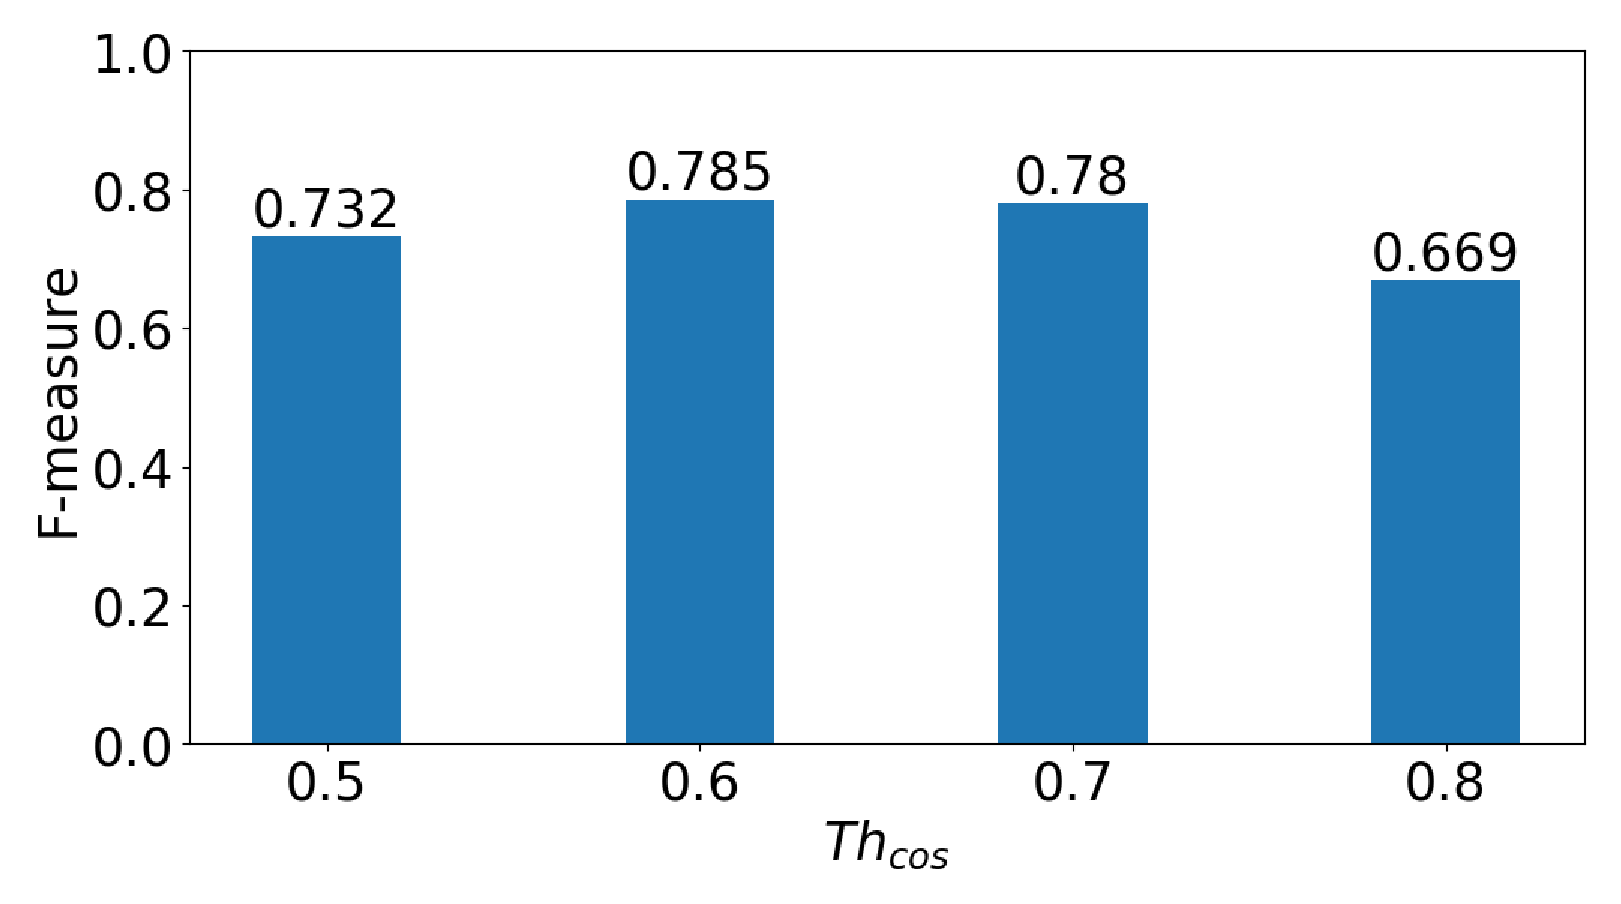
\includegraphics[keepaspectratio, scale=0.25]
                          {./figure/prob1_09_f.eps}}
      \end{minipage}

      \begin{minipage}{0.06\hsize}
        \hspace{0.01mm}
      \end{minipage}
 

    
    \end{tabular}
\caption{手法1によるアンカーの発話区間検出精度 ($Th_{time}=0.9$)}
\end{figure}
 
%手法1 1.0
\begin{figure}[H]
  \centering
    \begin{tabular}{c}
 
%----- recall -----
 
      \begin{minipage}{0.40\hsize}
        \centering
          \subfigure[Recall]{\includegraphics[keepaspectratio, scale=0.25]
                          {./figure/prob1_10_r.eps}}
      \end{minipage}

      \begin{minipage}{0.06\hsize}
        \hspace{0.01mm}
      \end{minipage}
 
%----- precision -----
 
      \begin{minipage}{0.40\hsize}
        \centering
          \subfigure[Precision]{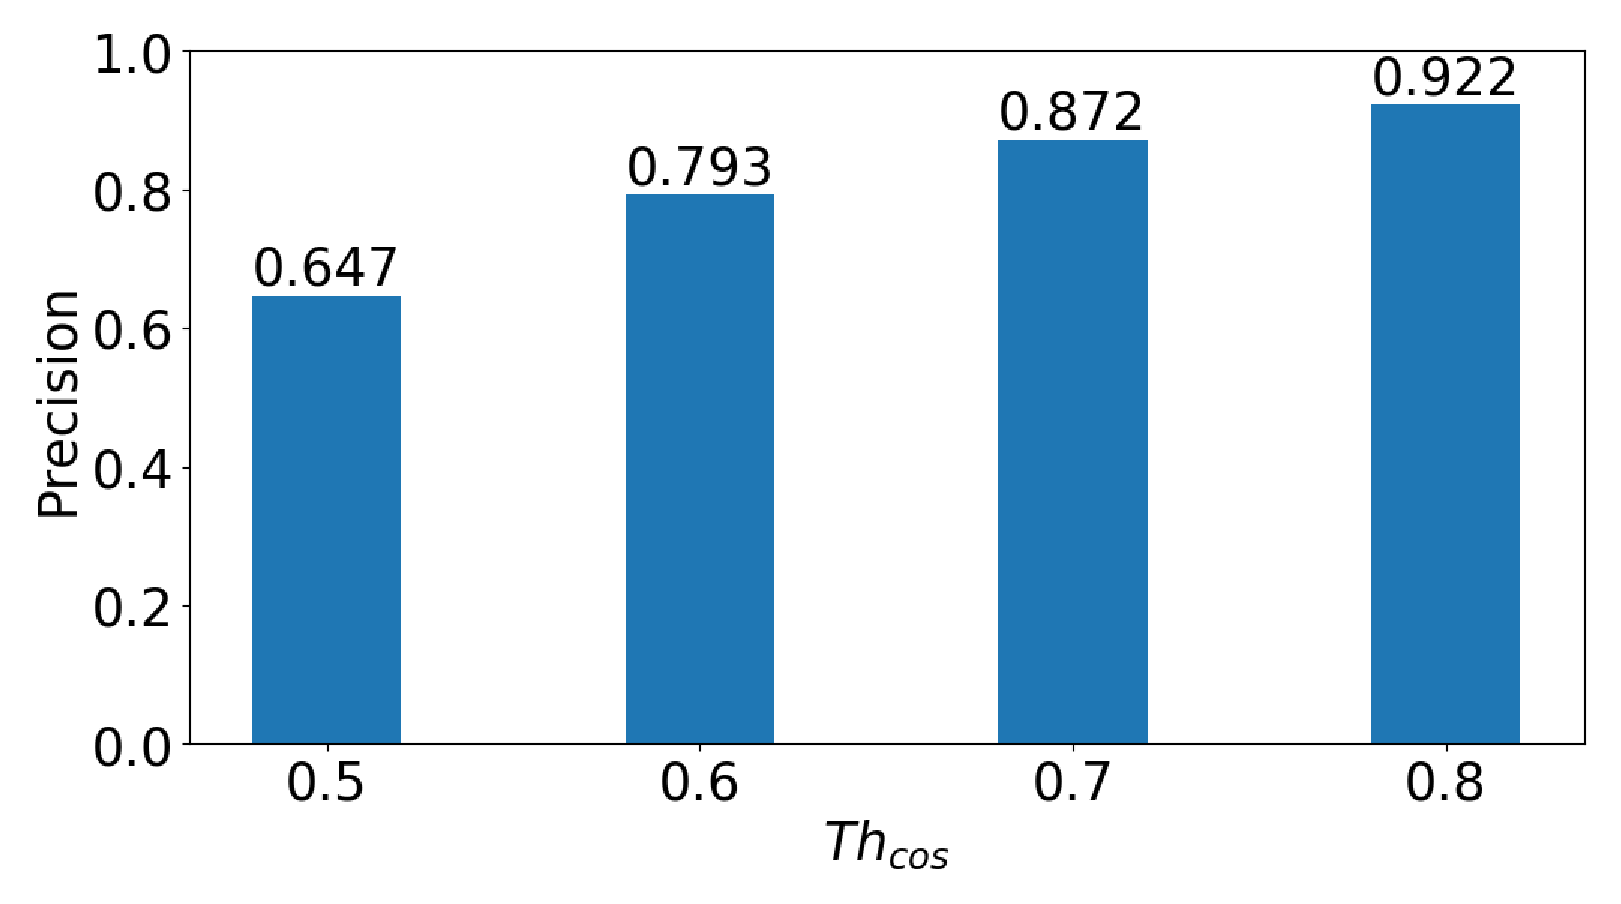
\includegraphics[keepaspectratio, scale=0.25]
                          {./figure/prob1_10_p.eps}}
      \end{minipage} \\

      \begin{minipage}{0.06\hsize}
        \vspace{5mm}
      \end{minipage} \\
 
 
%----- fmeasure -----
 
      \begin{minipage}{0.40\hsize}
        \centering
          \subfigure[F-measure]{\includegraphics[keepaspectratio, scale=0.25]
                          {./figure/prob1_10_f.eps}}
      \end{minipage}

      \begin{minipage}{0.06\hsize}
        \hspace{0.01mm}
      \end{minipage}
 

    
    \end{tabular}
\caption{手法1によるアンカーの発話区間検出精度 ($Th_{time}=1.0$)}
\end{figure} 

%手法1 1.1
\begin{figure}[H]
  \centering
    \begin{tabular}{c}
 
%----- recall -----
 
      \begin{minipage}{0.40\hsize}
        \centering
          \subfigure[Recall]{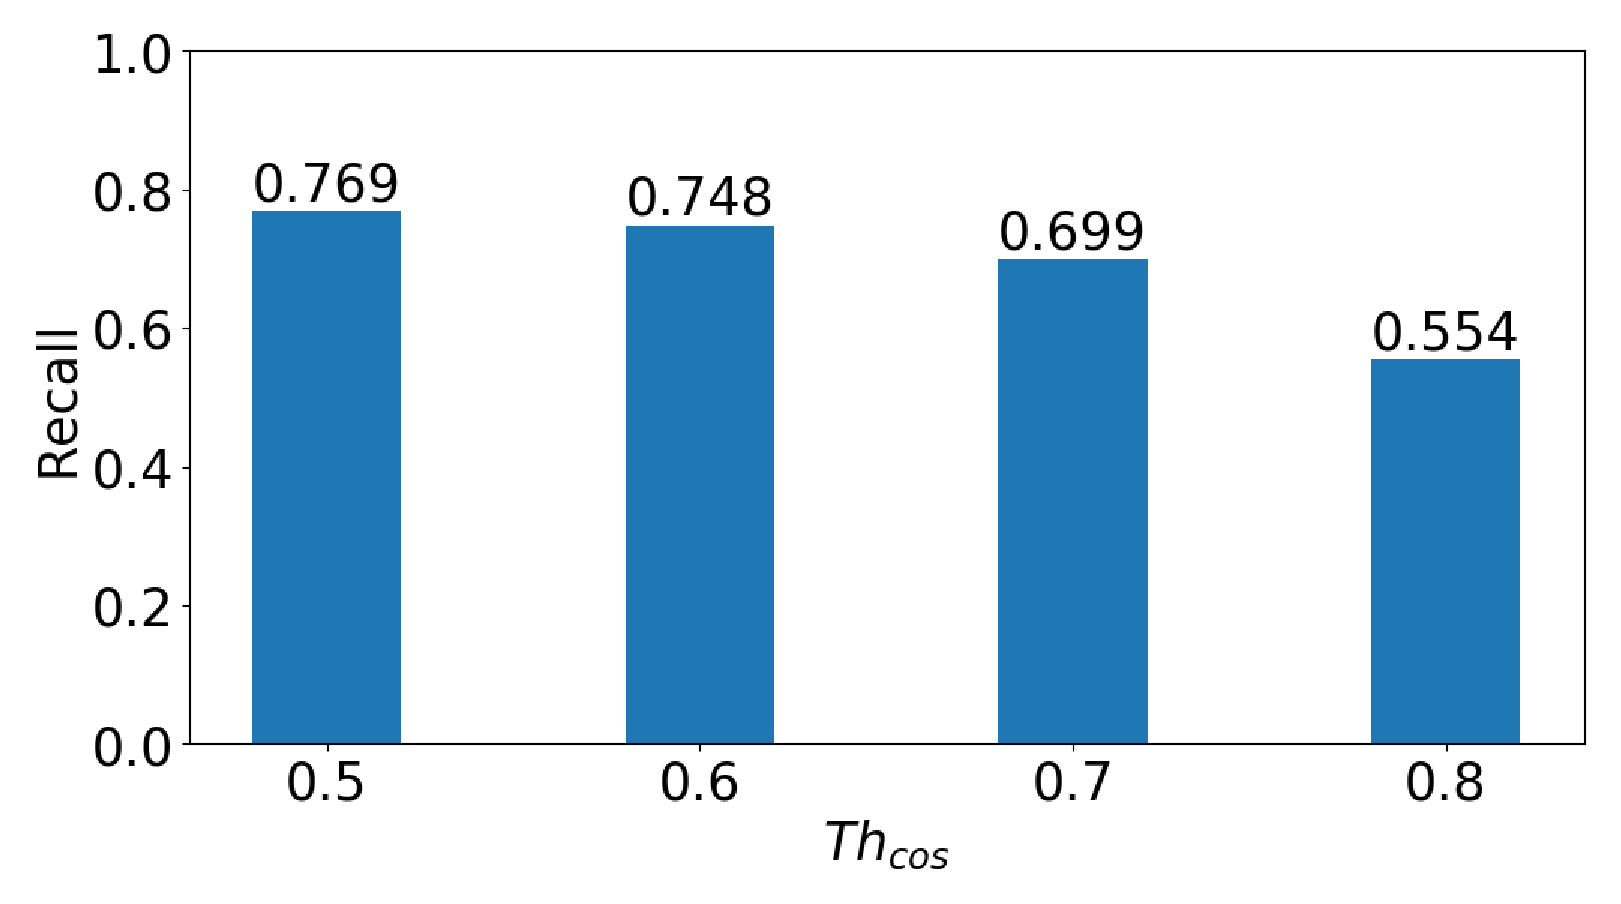
\includegraphics[keepaspectratio, scale=0.25]
                          {./figure/prob1_11_r.eps}}
      \end{minipage}

      \begin{minipage}{0.06\hsize}
        \hspace{0.01mm}
      \end{minipage}
 
%----- precision -----
 
      \begin{minipage}{0.40\hsize}
        \centering
          \subfigure[Precision]{\includegraphics[keepaspectratio, scale=0.25]
                          {./figure/prob1_11_p.eps}}
      \end{minipage} \\

      \begin{minipage}{0.06\hsize}
        \vspace{5mm}
      \end{minipage} \\
 
 
%----- fmeasure -----
 
      \begin{minipage}{0.40\hsize}
        \centering
          \subfigure[F-measure]{\includegraphics[keepaspectratio, scale=0.25]
                          {./figure/prob1_11_f.eps}}
      \end{minipage}

      \begin{minipage}{0.06\hsize}
        \hspace{0.01mm}
      \end{minipage}
    
    \end{tabular}
\caption{手法1によるアンカーの発話区間検出精度 ($Th_{time}=1.1$)}
\end{figure} 

%手法1 1.3
\begin{figure}[H]
  \centering
    \begin{tabular}{c}
 
%----- recall -----
 
      \begin{minipage}{0.40\hsize}
        \centering
          \subfigure[Recall]{\includegraphics[keepaspectratio, scale=0.25]
                          {./figure/prob1_13_r.eps}}
      \end{minipage}

      \begin{minipage}{0.06\hsize}
        \hspace{0.01mm}
      \end{minipage}
 
%----- precision -----
 
      \begin{minipage}{0.40\hsize}
        \centering
          \subfigure[Precision]{\includegraphics[keepaspectratio, scale=0.25]
                          {./figure/prob1_13_p.eps}}
      \end{minipage} \\

      \begin{minipage}{0.06\hsize}
        \vspace{5mm}
      \end{minipage} \\
 
 
%----- fmeasure -----
 
      \begin{minipage}{0.40\hsize}
        \centering
          \subfigure[F-measure]{\includegraphics[keepaspectratio, scale=0.25]
                          {./figure/prob1_13_f.eps}}
      \end{minipage}

      \begin{minipage}{0.06\hsize}
        \hspace{0.01mm}
      \end{minipage}
    
    \end{tabular}
\caption{手法1によるアンカーの発話区間検出精度 ($Th_{time}=1.3$)}
\end{figure}

%手法1 1.4
\begin{figure}[H]
  \centering
    \begin{tabular}{c}
 
%----- recall -----
 
      \begin{minipage}{0.40\hsize}
        \centering
          \subfigure[Recall]{\includegraphics[keepaspectratio, scale=0.25]
                          {./figure/prob1_14_r.eps}}
      \end{minipage}

      \begin{minipage}{0.06\hsize}
        \hspace{0.01mm}
      \end{minipage}
 
%----- precision -----
 
      \begin{minipage}{0.40\hsize}
        \centering
          \subfigure[Precision]{\includegraphics[keepaspectratio, scale=0.25]
                          {./figure/prob1_14_p.eps}}
      \end{minipage} \\

      \begin{minipage}{0.06\hsize}
        \vspace{5mm}
      \end{minipage} \\
 
 
%----- fmeasure -----
 
      \begin{minipage}{0.40\hsize}
        \centering
          \subfigure[F-measure]{\includegraphics[keepaspectratio, scale=0.25]
                          {./figure/prob1_14_f.eps}}
      \end{minipage}

      \begin{minipage}{0.06\hsize}
        \hspace{0.01mm}
      \end{minipage}
    
    \end{tabular}
\caption{手法1によるアンカーの発話区間検出精度 ($Th_{time}=1.4$)}
\end{figure}

%手法1 1.5
\begin{figure}[H]
  \centering
    \begin{tabular}{c}
 
%----- recall -----
 
      \begin{minipage}{0.40\hsize}
        \centering
          \subfigure[Recall]{\includegraphics[keepaspectratio, scale=0.25]
                          {./figure/prob1_15_r.eps}}
      \end{minipage}

      \begin{minipage}{0.06\hsize}
        \hspace{0.01mm}
      \end{minipage}
 
%----- precision -----
 
      \begin{minipage}{0.40\hsize}
        \centering
          \subfigure[Precision]{\includegraphics[keepaspectratio, scale=0.25]
                          {./figure/prob1_15_p.eps}}
      \end{minipage} \\

      \begin{minipage}{0.06\hsize}
        \vspace{5mm}
      \end{minipage} \\
 
 
%----- fmeasure -----
 
      \begin{minipage}{0.40\hsize}
        \centering
          \subfigure[F-measure]{\includegraphics[keepaspectratio, scale=0.25]
                          {./figure/prob1_15_f.eps}}
      \end{minipage}

      \begin{minipage}{0.06\hsize}
        \hspace{0.01mm}
      \end{minipage}
    
    \end{tabular}
\caption{手法1によるアンカーの発話区間検出精度 ($Th_{time}=1.5$)}
\end{figure}


%手法3 0.8
\begin{figure}[H]
  \centering
    \begin{tabular}{c}
 
%----- recall -----
 
      \begin{minipage}{0.40\hsize}
        \centering
          \subfigure[Recall]{\includegraphics[keepaspectratio, scale=0.25]
                          {./figure/prob3_08_r.eps}}
      \end{minipage}

      \begin{minipage}{0.06\hsize}
        \hspace{0.01mm}
      \end{minipage}
 
%----- precision -----
 
      \begin{minipage}{0.40\hsize}
        \centering
          \subfigure[Precision]{\includegraphics[keepaspectratio, scale=0.25]
                          {./figure/prob3_08_p.eps}}
      \end{minipage} \\

      \begin{minipage}{0.06\hsize}
        \vspace{5mm}
      \end{minipage} \\
 
 
%----- fmeasure -----
 
      \begin{minipage}{0.40\hsize}
        \centering
          \subfigure[F-measure]{\includegraphics[keepaspectratio, scale=0.25]
                          {./figure/prob3_08_f.eps}}
      \end{minipage}

      \begin{minipage}{0.06\hsize}
        \hspace{0.01mm}
      \end{minipage}
    
    \end{tabular}
\caption{手法3によるアンカーの発話区間検出精度 ($Th_{time}=0.8$)}
\end{figure}

%手法3 0.9
\begin{figure}[H]
  \centering
    \begin{tabular}{c}
 
%----- recall -----
 
      \begin{minipage}{0.40\hsize}
        \centering
          \subfigure[Recall]{\includegraphics[keepaspectratio, scale=0.25]
                          {./figure/prob3_09_r.eps}}
      \end{minipage}

      \begin{minipage}{0.06\hsize}
        \hspace{0.01mm}
      \end{minipage}
 
%----- precision -----
 
      \begin{minipage}{0.40\hsize}
        \centering
          \subfigure[Precision]{\includegraphics[keepaspectratio, scale=0.25]
                          {./figure/prob3_09_p.eps}}
      \end{minipage} \\

      \begin{minipage}{0.06\hsize}
        \vspace{5mm}
      \end{minipage} \\
 
 
%----- fmeasure -----
 
      \begin{minipage}{0.40\hsize}
        \centering
          \subfigure[F-measure]{\includegraphics[keepaspectratio, scale=0.25]
                          {./figure/prob3_09_f.eps}}
      \end{minipage}

      \begin{minipage}{0.06\hsize}
        \hspace{0.01mm}
      \end{minipage}
    
    \end{tabular}
\caption{手法3によるアンカーの発話区間検出精度 ($Th_{time}=0.9$)}
\end{figure}

%手法3 1.0
\begin{figure}[H]
  \centering
    \begin{tabular}{c}
 
%----- recall -----
 
      \begin{minipage}{0.40\hsize}
        \centering
          \subfigure[Recall]{\includegraphics[keepaspectratio, scale=0.25]
                          {./figure/prob3_10_r.eps}}
      \end{minipage}

      \begin{minipage}{0.06\hsize}
        \hspace{0.01mm}
      \end{minipage}
 
%----- precision -----
 
      \begin{minipage}{0.40\hsize}
        \centering
          \subfigure[Precision]{\includegraphics[keepaspectratio, scale=0.25]
                          {./figure/prob3_10_p.eps}}
      \end{minipage} \\

      \begin{minipage}{0.06\hsize}
        \vspace{5mm}
      \end{minipage} \\
 
 
%----- fmeasure -----
 
      \begin{minipage}{0.40\hsize}
        \centering
          \subfigure[F-measure]{\includegraphics[keepaspectratio, scale=0.25]
                          {./figure/prob3_10_f.eps}}
      \end{minipage}

      \begin{minipage}{0.06\hsize}
        \hspace{0.01mm}
      \end{minipage}
    
    \end{tabular}
\caption{手法3によるアンカーの発話区間検出精度 ($Th_{time}=1.0$)}
\end{figure}

%手法3 1.2
\begin{figure}[H]
  \centering
    \begin{tabular}{c}
 
%----- recall -----
 
      \begin{minipage}{0.40\hsize}
        \centering
          \subfigure[Recall]{\includegraphics[keepaspectratio, scale=0.25]
                          {./figure/prob3_12_r.eps}}
      \end{minipage}

      \begin{minipage}{0.06\hsize}
        \hspace{0.01mm}
      \end{minipage}
 
%----- precision -----
 
      \begin{minipage}{0.40\hsize}
        \centering
          \subfigure[Precision]{\includegraphics[keepaspectratio, scale=0.25]
                          {./figure/prob3_12_p.eps}}
      \end{minipage} \\

      \begin{minipage}{0.06\hsize}
        \vspace{5mm}
      \end{minipage} \\
 
 
%----- fmeasure -----
 
      \begin{minipage}{0.40\hsize}
        \centering
          \subfigure[F-measure]{\includegraphics[keepaspectratio, scale=0.25]
                          {./figure/prob3_12_f.eps}}
      \end{minipage}

      \begin{minipage}{0.06\hsize}
        \hspace{0.01mm}
      \end{minipage}
    
    \end{tabular}
\caption{手法3によるアンカーの発話区間検出精度 ($Th_{time}=1.2$)}
\end{figure}

%手法3 1.3
\begin{figure}[H]
  \centering
    \begin{tabular}{c}
 
%----- recall -----
 
      \begin{minipage}{0.40\hsize}
        \centering
          \subfigure[Recall]{\includegraphics[keepaspectratio, scale=0.25]
                          {./figure/prob3_13_r.eps}}
      \end{minipage}

      \begin{minipage}{0.06\hsize}
        \hspace{0.01mm}
      \end{minipage}
 
%----- precision -----
 
      \begin{minipage}{0.40\hsize}
        \centering
          \subfigure[Precision]{\includegraphics[keepaspectratio, scale=0.25]
                          {./figure/prob3_13_p.eps}}
      \end{minipage} \\

      \begin{minipage}{0.06\hsize}
        \vspace{5mm}
      \end{minipage} \\
 
 
%----- fmeasure -----
 
      \begin{minipage}{0.40\hsize}
        \centering
          \subfigure[F-measure]{\includegraphics[keepaspectratio, scale=0.25]
                          {./figure/prob3_13_f.eps}}
      \end{minipage}

      \begin{minipage}{0.06\hsize}
        \hspace{0.01mm}
      \end{minipage}
    
    \end{tabular}
\caption{手法3によるアンカーの発話区間検出精度 ($Th_{time}=1.3$)}
\end{figure}

%手法3 1.4
\begin{figure}[H]
  \centering
    \begin{tabular}{c}
 
%----- recall -----
 
      \begin{minipage}{0.40\hsize}
        \centering
          \subfigure[Recall]{\includegraphics[keepaspectratio, scale=0.25]
                          {./figure/prob3_14_r.eps}}
      \end{minipage}

      \begin{minipage}{0.06\hsize}
        \hspace{0.01mm}
      \end{minipage}
 
%----- precision -----
 
      \begin{minipage}{0.40\hsize}
        \centering
          \subfigure[Precision]{\includegraphics[keepaspectratio, scale=0.25]
                          {./figure/prob3_14_p.eps}}
      \end{minipage} \\

      \begin{minipage}{0.06\hsize}
        \vspace{5mm}
      \end{minipage} \\
 
 
%----- fmeasure -----
 
      \begin{minipage}{0.40\hsize}
        \centering
          \subfigure[F-measure]{\includegraphics[keepaspectratio, scale=0.25]
                          {./figure/prob3_14_f.eps}}
      \end{minipage}

      \begin{minipage}{0.06\hsize}
        \hspace{0.01mm}
      \end{minipage}
    
    \end{tabular}
\caption{手法3によるアンカーの発話区間検出精度 ($Th_{time}=1.4$)}
\end{figure}

%手法3 1.5
\begin{figure}[H]
  \centering
    \begin{tabular}{c}
 
%----- recall -----
 
      \begin{minipage}{0.40\hsize}
        \centering
          \subfigure[Recall]{\includegraphics[keepaspectratio, scale=0.25]
                          {./figure/prob3_15_r.eps}}
      \end{minipage}

      \begin{minipage}{0.06\hsize}
        \hspace{0.01mm}
      \end{minipage}
 
%----- precision -----
 
      \begin{minipage}{0.40\hsize}
        \centering
          \subfigure[Precision]{\includegraphics[keepaspectratio, scale=0.25]
                          {./figure/prob3_15_p.eps}}
      \end{minipage} \\

      \begin{minipage}{0.06\hsize}
        \vspace{5mm}
      \end{minipage} \\
 
 
%----- fmeasure -----
 
      \begin{minipage}{0.40\hsize}
        \centering
          \subfigure[F-measure]{\includegraphics[keepaspectratio, scale=0.25]
                          {./figure/prob3_15_f.eps}}
      \end{minipage}

      \begin{minipage}{0.06\hsize}
        \hspace{0.01mm}
      \end{minipage}
    
    \end{tabular}
\caption{手法3によるアンカーの発話区間検出精度 ($Th_{time}=1.5$)}
\end{figure}



% 付録がある場合
%\appendix
%\input{app}    % 付録

\chapter*{謝辞}

最後に,本研究および本修士論文作成にあたり暖かい御指導および適切な御助言をして頂いた松永 昭一教授,高田 寛之助教,山下 優博士に心より感謝いたします.

また,同研究室
博士前期(修士)課程2年の三浦 亮氏,
博士前期(修士)課程1年の入口 佳佑氏,堤 彬人氏,福永 慶士氏,
学士課程4年の平野 吉則氏,Zhang Tianzhi氏,
阿利 迪洋氏,梅野 直幹氏,古賀 光氏,増田 紗依氏,松本 優里奈氏,その他関係各位に心から感謝いたします.
    % 謝辞
\addcontentsline{toc}{chapter}{謝辞}

\begin{thebibliography}{99}     %文献数が10未満の時 {9}
\bibitem{1}Google
\end{thebibliography}
    % 参考文献
\addcontentsline{toc}{chapter}{参考文献} 

\end{document}
